\documentclass[10pt]{book}
\usepackage[utf8]{inputenc}
\usepackage[french]{babel}
\usepackage[T1]{fontenc}
\usepackage{verbatim}
\usepackage{graphicx}
\usepackage{amsmath}
\usepackage{amssymb}
\usepackage{amsthm}
\usepackage{textcomp}
\usepackage{csquotes}
\usepackage{fullpage}
\usepackage{eurosym}
\setcounter{secnumdepth}{5}
\author{Contzen Laurent}
\title{Introduction à la macroéconomie : Résumé}

\begin{document}
\maketitle
\tableofcontents
\newpage
\chapter{Qu'est ce que la macroéconomie?}
\section{Introduction : une définition}
Macroéconomie : \og Discipline qui a pour objet d'analyser l'économie d'un pays d'un point de vue global \fg. Cette définition appelle deux commentaires :
\begin{itemize}
  \item Analyse globale $\rightarrow$ les variables d'intérêt seront des agrégats.
  \item Démarche scientifique.
\end{itemize}

\section{La macroéconomie : une discipline scientifique}

\subsection{Évolution de la macroéconomie en tant que discipline}

\subsubsection{Une discipline jeune}
La macroéconomie est née avec la révolution Keynésienne dans les années 30. Le livre de Keynes qui sert de référence est \textit{Théorie générale de l'emploi, de l'intérêt et de la monnaie}. Avant lui, de nombreux économistes s'intéressaient aux phénomènes globaux en les appréhendant à l'échelle des nations. \\
En opposition aux analyses en vogue à l'époque, la théorie keynésienne va proposer une triple rupture :
\begin{itemize}
  \item En rupture avec l'analyse néoclassique, Keynes s'intéresse à des agrégats et à des comportements \textit{globaux} (Produit national, consommation, investissement, ...). Il impose aussi un raisonnement où ce ne sont pas les prix qui ajustent l'offre et la demande sur des marchés mais dans lequel l'équilibre se définit en terme de flux. On peut critiquer cette perspective car elle ne repose pas sur le comportement observable d'individus mais se prête à la quantification $\rightarrow$ ça a permis le développement de la comptabilité nationale.
  \item Keynes se concentre sur un nouvel objet d'étude : le \textit{niveau d'activité}. Il montre que le plein emploi n'est pas l'état normal de l'économie de marché $\rightarrow$ il faut étudier ce qui détermine le niveau de l'emploi.
  \item Il devient possible de réfléchir aux politiques économiques susceptibles d'influencer le niveau d'activité. Keynes va suggérer qu'une politique bien menée peut atténuer les fluctuations conjoncturelles. Entre le laisser-faire et la planification il propose une troisième solution qui consiste à confier à l'état la gestion de l'activité globale dans une économie de marché. L'instrument privilégié est le budget de l'état qui peut relancer l'activité en augmentant ses dépenses $\rightarrow$ \textit{politique budgétaire}
\end{itemize}
La théorie keynésienne propose donc des solutions à un problème majeur dont les théories précédentes sont incapables de rendre compte $\rightarrow$ succès politique et scientifique.

\subsubsection{Une discipline en débat}
Au lendemain de la seconde guerre mondiale, la théorie keynésienne tient une position quasiment hégémonique sur la macroéconomie. Elle va déboucher sur un consensus appelé la \textit{synthèse néoclassique}. Ce consensus scientifique reposait fondamentalement sur les idées keynésiennes traduites et formalisées et était complété par des relations issues de la théorie néoclassique et de travaux statistiques qui permettaient d'intégrer les mouvements de prix. Dans tous les cas on considérait qu'une politique économique judicieuse permettait de réduire efficacement les fluctuations conjoncturelles $\rightarrow$ la recherche se concentrait sur l'amélioration des théories et des modèles de la synthèse. \\ \\
Mais les conclusions de la théorie keynésienne vont susciter des critiques de plus en plus vives. De celles ci va émerger la \textit{critique monétariste}. Celle ci se base sur trois arguments principaux :
\begin{itemize}
  \item Les monétaristes ont souligné l'efficacité de la politique monétaire comme instrument de politique économique. Elle consiste à jouer sur la quantité de monnaie en circulation et les taux d'intérêt pour influencer l'activité, alors que la théorie keynésienne privilégiait la politique budgétaire.
  \item Dans les années 50 et 60 les économiste de la synthèse considéraient que grâce à la politique macroéconomique il était possible d'arbitrer en permanence entre chômage et inflation. Cette conviction s'appuyait sur la courbe de Phillips. Les monétaristes se sont opposés à l'idée qu'une telle relation puisse exister car pour eux elle supposait une forme d'illusion monétaire permanente. Selon eux, toute tentative d'exploiter cette relation ne pouvait de plus déboucher que sur de l'inflation, sans effet sur le chômage. L'apparition de la \textit{stagflation} (chômage et inflation) dans les années 70 participa à populariser leurs arguments.
  \item Enfin, pour les monétaristes, toute tentative de limiter les fluctuations par la politique économique était vouée à l'échec. Ils considéraient que nos connaissances du fonctionnement de l'économie sont trop imparfaites pour prétendre gérer efficacement le cycle économique. Surtout si on rajoute le temps de réaction des autorités.
\end{itemize}
Par conséquent, il vaut mieux avoir recours à des \textit{règles} de politique économique. Friedman proposait par exemple que la politique monétaire ait pour principe de maintenir constant le taux de croissance de la masse monétaire quelles que soient les circonstances. \\
Malgré tout, les monétaristes acceptaient dans une large mesure la théorie keynésienne. Leur critique portait plus sur sa capacité à formuler des conseils de politique économique que sur sa pertinence théorique. \\ \\
Dans les années 70 en revanche une critique radicale des analyses keynésiennes allait apparaître. Ce seront les \textit{nouveaux classiques}. Ceux ci sont les économistes qui ont remis en cause la théorie keynésienne en s'en prenant à ses fondements théoriques. Ils s'opposent à l'interventionnisme keynésien et critiquent notamment le manque de fondements micro-économiques de la théorie keynésienne. Ils accusent cette dernière de ne pas correctement prendre en compte les anticipations des agents et leurs effets sur leurs décisions présentes. Ils proposent de bâtir les analyses macroéconomiques sur l'hypothèse \textit{d'anticipations rationnelles} $\rightarrow$ on parle du courant des anticipations rationnelles. Cette hypothèse consiste à supposer que les agents économiques fondent leurs anticipations de l'évolution des variables économiques qui les concernent aussi rationnellement que possible, en tenant compte de toute l'information disponible. Ceci remet en cause les principales conclusions keynésiennes en termes d'efficacité des politiques économiques puisque si les agents anticipent la politique économique, ils s'y adaptent instantanément et celle ci ne peut avoir un effet que si elle surprends le secteur privé. \\

\subsection{Questions méthodologiques}
\subsubsection{Ce qu'on attends de la macroéconomie}
L'économie est une science sociale qui s'est constituée au cours du temps pour conseiller les décisions des gouvernements, c'est pourquoi on parle d'\textit{économie politique}. Ce que le public et les gouvernements attendent de la macroéconomie est de formuler des jugements et de proposer des politiques à mettre en oeuvre. \\
La macroéconomie ne peut émettre directement des recommandations de politique économique. Elle doit d'abord passer par une étape au cours de laquelle elle va avoir pour objet d'expliquer les phénomènes économiques, ce qui relève de ce qu'on appelle une \textit{démarche positive}. Elle consiste à établir des relations entre certains faits et donc à fournir des explications, des théories. L'étape qui consiste à formuler des recommandations relève d'une \textit{démarche normative}. Dans notre cas, notre démarche sera guidée par des jugements de valeurs (e.g. l'amélioration des niveaux de vie est souhaitable alors que l'inflation ne l'est pas) et sur des modèles.
\subsubsection{L'importance de la modélisation}
La théorie macroéconomique repose largement sur des modèles (expression d'une théorie sous la forme d'un ensemble d'hypothèses qui relie entre elles des variables jugées pertinentes). La plupart du temps les modèles macroéconomiques sont formalisés et on y distingue alors deux types de variables : 
\begin{itemize}
  \item les \textit{variables endogènes} qui sont celles que le modèle va expliquer
  \item les \textit{variables exogènes} qui sont celles qui sont considérées comme ``données''.
\end{itemize}
Le but du jeu est d'expliquer les variations des variables endogènes par celles de certaines variables exogènes. Les autres variables exogènes sont appelées des \textit{paramètres}. Pour cela, on est souvent amenés à simplifier la réalité pour la modéliser en ne gardant que les informations pertinentes. La macroéconomie utilise une variété de modèles qui peuvent être complémentaires, mais tous sont confrontés à la même \textit{contrainte de bouclage} qui impose de tenir compte du fonctionnement et des interactions de tous les marchés qui constituent le modèle. Il n'est pas possible de s'intéresser à un marché sans tenir compte de ses effets sur les autres marchés. On doit donc toujours raisonner en termes d'\textit{équilibre global} de l'économie. Certaines \textit{égalités comptables} doivent en particulier être respectées sans quoi le modèle sera incohérent.

\section{Les principaux agrégats}
Puisque la macroéconomie étudie les phénomènes économiques d'un point de vue agrégé elle doit utiliser des données elles aussi agrégées, ce sont les agrégats et c'est la \textit{comptabilité nationale} qui permet de les construire. On va se concentrer ici sur les agrégats qui mesurent les principaux objectifs de la politique économique (le  revenu, le niveau des prix et le chômage) qui correspondent aussi à trois des côtés du \textit{carré magique} de la politique économique et définir une distinction essentielle, celle qui oppose les variables de flux aux variables de stock.
\subsection{Flux et stocks}
La distinction entre les deux peut être définie simplement : 
\begin{itemize}
  \item \textit{Flux} : Variable qui se mesure sur un intervalle de temps.
  \item \textit{Stock} : Variable qui se mesure à un instant donné.
\end{itemize}
Un stock peut être vu comme une accumulation de flux. Par exemple, la dette publique (stock) est constituée des déficits passés (flux). Pour s'en convaincre, il suffit de partir de la dernière dette en date ($t$), qui est égale à la dette se la période précédente à laquelle s'ajoute le déficit de l'année :
$$ Dpub_t = Dpub_{t-1} + déficit_t $$
Mais on peut écrire la même chose pour la période précédente ($t-1$) :
$$ Dpub_{t-1} = Dpub_{t-2} + deficit_{t-1} $$
$$ \Rightarrow Dpub_{t} = deficit_t + deficit_{t-1} + Dpub_{t-2}$$
En remontant le temps de la même façon, on obtient que :
$$Dpub_t = deficit_t + deficit_{t-1} + deficit_{t-2} + ... + deficit_{t-n+1} + Dpub_{t-n}$$
et en remontant suffisamment loin dans le temps on trouvera bien une période $t-n$ où la dette publique était nulle. La dette est dont bien la somme des déficits passés. \\
On peut à l'inverse exprimer les flux en fonction des stocks : si on connaît le montant de la dette de cette année et de l'année dernière, on pourra déduire le montant du déficit en calculant la différence entre les deux :
$$deficit_t = Dpub_t -  Dpub_{t-1}$$
Plus généralement, on peut écrire que les flux correspondent aux variations des stocks : 
\begin{center}
  \fbox{$\Delta STOCK = FLUX$}
\end{center}
\subsection{La mesure du revenu}
Il n'existe pas une mesure unique du revenu mais plusieurs. La plus utilisée en macroéconomie est le \textit{produit intérieur brut}.
\subsubsection{Le PIB nominal}
\paragraph{Définition}
Le PIB a une définition unique mais peut être calculé de trois façons différentes cohérentes entre elles. \\
\textit{PIB} : Valeur monétaire de l'ensemble des biens et services finaux produits sur le territoire d'un pays pendant une période donnée. \\
Quelques remarques : 
\begin{itemize}
  \item Ensemble des biens et services $\rightarrow$ Tout ce qui est produit comme richesse dans l'économie sauf les activités illicites et domestiques.
  \item Pendant une période donnée $\rightarrow$ C'est un flux.
  \item Bien et services finaux $\rightarrow$ On exclut les consommations intermédiaires sauf si ils sont stockés. Dans ce cas ils sont considérés comme une consommation finale pour la période courant et seront déduits du PIB au moment où ils seront déstockés.
  \item Produits sur le territoire $\rightarrow$ C'est la production des \textit{unités résidentes} qui compte. Un belge qui travaille au Lux ne fait pas augmenter le PIB belge mais le PIB luxembourgeois et inversement.
  \item Valeur monétaire $\rightarrow$ On exprime tout dans une unité commune
\end{itemize}
On mesure donc la valeur des biens grâce à leur prix, c'est pourquoi on parle de \textit{PIB nominal}. Le PIB mesure la production totale d'un pays $\rightarrow$ il dépends de sa taille. C'est pourquoi on va souvent utiliser le \textit{PIB par habitant} (ou par tête ou per capita) qui est le PIB  divisé par le nombre d'habitants.
\paragraph{Les trois modes de calcul du PIB} 
\begin{itemize}
  \item \textbf{Optique de la production :} \\
    C'est l'application directe de la définition du PIB. On cherche à mesurer la richesse produite dans l'économie. Dans ce cas, le PIB est la somme des valeurs ajoutées :    
    \begin{center}
      \fbox{$PIB = \Sigma VA$}
    \end{center}
    La \textit{valeur ajoutée} d'un bien correspond à la différence entre la valeur du bien ou du service et la valeur des inputs matériels qui ont été nécessaires pour le réaliser. \\
    Calculer le PIB à partir de la somme des VA permet d'éviter de compter deux fois les inputs matériels.
  \item \textbf{Optique des dépenses :} \\
    Le PIB mesure le revenu d'une année mais ce revenu va aussi être dépensé. Or au niveau du pays dans son ensemble la dépense va être égale au revenu. On va donc mesurer la richesse au moment où elle va être utilisée. On dit que le PIB est égal à la somme des \textit{demandes finales}. 
    \begin{center}
      \fbox{$PIB = \Sigma Demandes~Finales$}
    \end{center}
    %Les demandes finales sont la consommation, les investissements, les dépenses publiques et les exportations auxquelles on soustrait les importations.%
    Le PIB calculé par l'optique de la dépense est au final égal à la somme de la consommation finale, de l'investissement (ou formation brute de capital fixe), de la variation des stocks et des exportations nettes.
  \item \textbf{Optique des revenus :} \\
    Lorsque la richesse a été produite elle doit être redistribuée, on va donc la mesurer en calculant la somme des revenus des facteurs de production (salaires, revenus du capital, ...).  
    \begin{center}
      \fbox{$PIB = \Sigma revenus~des~facteurs$}
    \end{center}
\end{itemize}
Les trois mesures donnent exactement le même résultat. \\
Ce qu'on calcule comme ça est le \textit{PIB au prix du marché}. On peut aussi calculer le \textit{PIB au coût des facteurs} en soustrayant les impôts et en réintégrant les subventions au \textit{PIB au prix du marché} :
$$PIB_{cf} = PIB_{pm} - impots~directs + subventions$$
Le $PIB_{cf}$ est une meilleure mesure de la production que le $PIB_{pm}$ car il est insensible aux variations des prélèvements et subventions publics. 
\paragraph{L'identité comptable fondamentale}
A partir de la définition du PIB on peut déduire une \textit{identité comptable}, c'est à dire une égalité qui sera par construction toujours vraie. Tout modèle qui ne la respecte pas est par définition incohérent. \\
Dans une économie fermée sans état, le PIB est utilisé soit pour la consommation, soit pour l'investissement. On peut alors écrire :
$$ Y \equiv C + I $$
On va compléter ceci par une seconde égalité qui définira l'épargne. Par analogie avec le cas d'un consommateur individuel , l'épargne est définie par la différence entre le revenu et la consommation. Or on sait que le PIB est aussi égal à la somme des revenus. Par conséquent :
$$  S \equiv Y-C $$
Si on combine les deux définitions on arrive à
$$ S = (C + I) - C $$ 
\begin{center}
  \fbox{$\Rightarrow S = I$}
\end{center}
C'est l'identité comptable fondamentale en économie fermée sans état. Elle est toujours vraie. Elle traduit le fait que le production est répartie entre les consommateurs et les entreprises. Ce qui n'est pas consommé et donc épargné peut être investi et vice versa. \\ \\
On peut par le même raisonnement définir l'identité comptable fondamentale dans le cas d'une économie ouverte avec un état en partant de la définition du PIB : 
$$ Y \equiv C + I + G + NX $$
On définit toujours l'épargne comme la différence entre le revenu et la consommation. Il faut à présent soustraire un prélèvement important sur le revenu brut avant d'obtenir l'épargne : les impôts.
$$ S = Y - C - T$$
$$ \Leftrightarrow S = (C + I + G + NX) - C - T$$
Ce qui nous permet d'obtenir une identité comptable intéressant : 
\begin{center}
  \fbox{$(S-I) + (T-G) = NX$}
\end{center}
Ce qui revient à dire que la capacité de financement est égale au solde de la balance commerciale. En d'autres termes, l'excédent commercial est égal à la somme de l'épargne privée et de l'épargne publique. A l'inverse, si l'excédent budgétaire est négatif, càd si on observe un déficit budgétaire, et si l'épargne privée ne le compense pas, on observera aussi un déficit commercial. C'est pourquoi on parle de \textit{twin deficits}.
\subsubsection{La comparaison des PIB dans le temps et l'espace}
Les comparaisons de PIB dans le temps et l'espace sont impossibles avec le PIB nominal car le PIB agrège des quantités de biens différents en les pondérant par leurs prix, or les prix évoluent au cours du temps et diffèrent d'un pays à un autre. C'est pourquoi il existe aussi le PIB réel.
\paragraph{Le PIB réel}
Lorsqu'on souhaite comparer les PIB de deux années différentes, on souhaite comparer la richesse produite pendant ces deux années. Or entre ces deux années les prix ont forcément changé. ceci peut être dû à l'inflation et/ou à des variations de prix relatifs, mais une tonne de blé reste une tonne de blé quel que soit son prix. On va donc trouver un moyen de neutraliser l'effet des mouvement de prix, ce qui va permettre de se faire une véritable idée de l'évolution des quantités produites. \\
La méthode est simple : on choisit une année de référence, l'\textit{année de base}, et on utilise les prix de cette année là pour les appliquer aux quantités produites pendant les autres années. On obtient ainsi le PIB réel de chaque année aux prix de l'année de base. \\
\textit{PIB réel, en volume} ou \textit{à prix constants} : production de biens et services valorisée aux prix de l'année de base. \\
Les PIB réels des différentes années sont à présent comparables puisque les différences entre eux ne sont plus dues qu'à l'évolution des quantités produites. L'augmentation du PIB nominal surestime toujours celle du PIB réel en période d'inflation et la sous-estime en période déflation. \\
Lorsque l'on a calculé le PIB réel et le PIB nominal, on peut en déduire le \textit{déflateur du PIB} : 
\begin{center}
  \fbox{$deflateur~du~PIB = \frac{PIB~nominal}{PIB~reel}$}
\end{center}
Ce déflateur mesure l'évolution des prix entre l'année de base et l'année courante, c'est donc une mesure de l'inflation.
\paragraph{Le PIB à parité des pouvoirs d'achat}
Pour comparer les PIB dans l'espace il y a aussi des problèmes : les prix peuvent différer d'un pays à l'autre, et dans le cas d'une comparaison entre deux pays qui n'utilisent pas la même monnaie il faut passer par un taux de change qui peut fluctuer de manière importante. Tout ceci peut fausser de façon significative les comparaisons internationales de revenu. Par conséquent, en comparant les PIB nominaux on obtient une idée faussée des différences de revenu d'un pays à l'autre. Pour résoudre ce problème, on utilise une monnaie fictive qui respecte la \textit{parité des pouvoirs d'achats} et on calcule des taux de change pour cette monnaie fictive. Ces derniers sont tels que cette monnaie permette d'acheter la même quantité de biens dans tous les pays. On obtient ainsi par exemple des Dollars PPA. \\
Il faut garder à l'esprit que des écarts de PIB très faibles ne sont en général pas significatifs car il y a trop d'approximations dans les calculs et d'imprécisions dans les données.
\paragraph{D'autres mesures du revenu}
Au lieu du PIB on entends souvent parler du PNB ou Produit National Brut. Les deux agrégats sont très proches mais il existe une différence de taille entre les deux qui apparaît en comparant les définitions des deux : \\
\textit{PNB} : Valeur monétaire de l'ensemble des biens et services finaux produits par les facteurs de production nationaux pendant une période donnée. \\
Ici ce qui compte est la nationalité des détenteurs des facteurs de production et non le lieu de leur activité. Un belge qui travaille au luxembourg fait augmenter le PNB belge mais pas le PNB luxembourgeois. \\
Depuis l'adoption des nouvelles normes de comptabilité nationale dans l'UE le \textit{Revenu National Brut} a remplacé le PNB. On obtient facilement le PNB (RNB) à partir du PIB :
$$PNB(RNB)~=~PIB~+~revenus~des~facteurs~recus~du~reste~du~monde$$
$$~~~~~~~~~~~~~~-~revenus~des~facteurs~verses~au~reste~du~monde$$
En Belgique la différence entre le PNB et le PIB est très faible (environ $1\%$) mais dans les pays de forte émigration le PNB est supérieur au PIB car une grande partie leurs nationaux travaillent à l'étranger, de même les pays qui possèdent un nombre important d'entreprises à l'étranger auront un PNB supérieur au PIB. Inversement les pays sur le territoire desquels opèrent des entreprises détenues par des étrangers auront un PIB supérieur à leur PNB. \\
Par ailleurs, le PIB surestime la richesse réellement disponible pendant une année. En effet, une partie du stock de capital s'est usée et a vieilli. Une partie de la production totale a donc du être consacrée au remplacement du capital devenu hors d'usage. C'est ce que mesurent les \textit{amortissements}. En retranchant les amortissements du PIB on obtient le \textit{Produit Intérieur Net} :
$$Produit~Interieur~Net~=~PIB~-~Amortissements$$
Le PIN mesure donc la richesse créée nette de celle qui a été détruite au cours de la production. C'est donc une meilleure mesure du revenu d'un pays. C'est pourquoi on l'appelle également \textit{revenu national}. \\
Il faut se méfier de l'utilisation du PIB ou du PNB par habitant pour mesurer le bien-être d'un pays : 
\begin{itemize}
  \item Le PIB par habitant est une moyenne et peut cacher des disparités importantes au sein de la population.
  \item Le PIB ne prends pas en compte la pollution.
  \item Le PIB ne tient pas compte de l'augmentation du temps de loisir et la diminution du temps de travail.
  \item Le PIB ne tient pas compte de l'utilisation des ressources naturelles qui peuvent pourtant s'épuiser.
\end{itemize}
Pour pallier à ces lacunes on a développé des mesures alternatives : 
\begin{itemize}
  \item L'\textit{Indice de Développement Humain} (IDH) est un indice composite qui dépends du revenu par habitant mais tient compte de la décroissance de l'utilité marginale du revenu, de l'espérance de vie, du taux d'alphabétisation et du taux de scolarisation. Bien que le  classement des pays en fonction de leur IDH soit globalement proche de celui obtenu à partir de leur PIB par tête on observe des différences.
  \item Certains ont proposé l'idée d'un \textit{PIB vert} ou \textit{écologique} qui les intégrerait.
  \item Les US ont aussi introduit des \textit{comptes écologiques} ou \textit{comptes verts} dans leurs comptabilité nationale.
\end{itemize}

\subsection{L'inflation}
La lutte contre l'inflation est un objectif de la politique économique. La BCE a chiffré cet objectif en indiquant juste avant le lancement de l'euro qu'elle cherchait à atteindre un taux d'inflation inférieur à $2\%$. Pour mesurer cet objectif on peut utiliser soit l'\textit{Indice des prix à la consommation} (IPC) soit le déflateur du PIB.
\subsubsection{L'indice des prix à la consommation}
On le construit en trois étapes : 
\begin{itemize}
  \item Définir le panier du consommateur moyen.
  \item Calculer le prix de ce panier de biens à intervalle régulier.
  \item Calculer l'indice des prix en rapportant le prix courant du panier à celui d'une année de base.
\end{itemize}
Comme l'IPC est un rapport entre deux variables mesurées dans la même unité il n'a lui-même pas d'unité. \\
L'IPC ne mesure pas directement l'inflation. Pour cela il faut calculer le taux de variation annuel de l'IPC. On peut alors définir le taux d'inflation : \\
\textit{Taux d'inflation} : Taux de variation de l'IPC sur une période donnée. \\
Depuis 2004 on peut ajuster tous les deux ans la liste des produits contenus dans chaque catégorie composant le panier du consommateur moyen. Bien que sa construction soit en principe simple, l'IPC admet trois lacunes principales : 
\begin{itemize}
  \item Problème de \textit{substitution} : L'IPC repose sur l'hypothèse que le panier de biens représentatifs est invariant. Or, si les prix évoluent les consommateurs vont modifier la répartition de leur budget en substituant aux biens dont le prix a augmenté des biens moins coûteux. La composition du panier va alors s'éloigner de celle de la consommation effective.
  \item Problème des \textit{biens nouveaux} : La composition du panier étant en principe fixée une fois pour toutes, il ne peut prendre en compte les biens nouveaux, alors que l'évolution de leurs prix peut être sensiblement différente de celle des autres biens.
  \item Problème de l'\textit{évolution de la qualité} des biens : grâce au progrès technique la qualité des biens tend en général à s'améliorer. On remplace sans s'en rendre compte des biens anciens par des biens de meilleure qualité. La composition du panier n'est donc pas constante dans le temps.
\end{itemize}
Ces trois problèmes créent un biais dans le même sens : l'IPC tend à surestimer l'inflation. C'est l'\textit{effet Boskin}. Un taux de variation de l'IPC de $1\%$ correspondrait à un inflation nulle. \\
Par ailleurs, on essaye de tenir compte de l'évolution de la qualité des biens grâce à la méthode des \textit{prix hédoniques} qui consiste à corriger l'augmentation de la qualité des biens, en tenant compte de ce que les consommateurs sont prêts à payer pour l'écart de qualité.
\subsubsection{La mesure de l'inflation grâce au déflateur du PIB}
Compte tenu des lacunes de l'IPC, il est utile de le compléter par une autre mesure de l'inflation. C'est une des utilisations du déflateur du PIB. Comme l'IPC, le déflateur est un indice et n'a pas d'unité en soi. En revanche, sa variation donne aussi une indication de l'évolution des prix $\rightarrow$ les évolutions de l'IPC et du déflateur seront proches. Il existe cependant deux différences importantes : 
\begin{itemize}
  \item Le déflateur concerne l'évolution de tous les prix des biens et services produits sur le territoire alors que l'IPC n'intègre que le prix des biens consommés par les consommateurs présents sur ce territoire. L'IPC n'intègre donc pas le prix des commandes publiques alors que le déflateur le fait. A l'inverse, l'IPC intègre le prix des biens importés alors que le déflateur ne le fait pas.
  \item On a vu que la composition du panier de biens sur lequel est calculé l'IPC n'est que rarement révisée alors que la composition du PIB s'ajuste en permanence aux quantités produites. Le déflateur est donc calculé à partir de quantités qui s'adaptent en permanence.
\end{itemize}
Par conséquent, les taux d'inflation mesurés à partir de l'IPC et du déflateur se ressemblent mais ne coïncident pas. Par exemple, le déflateur va moins refléter un choc pétrolier que l'IPC.

\subsection{Le chômage}
\subsubsection{La distinction entre chômage, inactivité et emploi}
A tout instant on peut classer les adultes selon trois catégories : 
\begin{itemize}
  \item Ceux qui ont un emploi, i.e. une activité rémunérée.
  \item Les chômeurs qui n'ont pas d'activité rémunérée.
  \item Les inactifs, c'est à dire ceux qui ont une activité non rémunérée (étudiants, femmes/hommes au foyer, ...).
\end{itemize}
La \textit{population active} regroupe les personnes qui occupent un emploi et les chômeurs. C'est par rapport à celle-ci qu'on mesure le taux de chômage : \\
\textit{Taux de chômage} = 100 $\times$ nombre de chômeurs / population active. \\
Il ne faut pas confondre le taux de chômage avec le taux d'activité de la population qui mesure la part des actifs dans la population adulte, c'est à dire en âge de travailler : \\
\textit{Taux d'activité} = 100 $\times$ population active / population adulte.
\subsubsection{La difficulté de mesurer le chômage}
Pour mesurer le chômage, il est nécessaire de tracer une limite nette entre activité, inactivité et chômage, afin de pouvoir classer les individus dans l'une de ces catégories. Cependant, certaines situations sont très floues : 
\begin{itemize}
  \item Une personne qui travaille à temps partiel involontaire occupe un emploi mais est touchée partiellement par le chômage.
  \item Un chômeur en formation peut être considéré comme un actif, puisqu'il est chômeur, ou comme un inactif, puisqu'il suit une formation.
  \item \ldots
\end{itemize}
Il est donc nécessaire de donner une définition opérationnelle du chômage. Une première définition consiste à considérer comme chômeurs tous les individus qui sont inscrits à l'ONEM, mais cette définition pose aussi des problèmes : tous les chômeurs ne sont pas inscrits, certains travailleurs au noir sont inscrits et les systèmes de prise en charge de chômeurs diffèrent d'un pays à un autre, ce qui rends délicates les comparaisons internationales. On retiendra plutôt la définition du Bureau International du Travail : \\
\textit{Chômeur au sens du B.I.T.} : Toute personne en âge de travailler, sans emploi, immédiatement disponible et à la recherche d'un emploi ou en ayant trouvé un qui commence ultérieurement. \\
Plus précisément, le B.I.T. définit une personne en âge de travailler comme ayant 15 ans ou plus, le fait d'être sans emploi comme celui de ne pas avoir travaillé, ne serait-ce qu'une heure, durant une semaine de référence et le fait d'être immédiatement disponible comme celui de pouvoir prendre un emploi dans les 15 jours.

\part{La croissance}
\chapter*{Introduction}
Lorsqu'un macroéconomiste parle de la croissance, et à fortiori de la théorie de la croissance, il utilise le terme dans un sens plus restrictif que juste la croissance de la production, dont la définition pourrait être : \\
\textit{Croissance} : augmentation pendant une période longue du produit d'un pays. \\
La croissance est donc considérée comme un phénomène de long terme. elle concerne les tendances longues, on parlera parfois de ``trends''. L'ordre de grandeur est au moins celui d'une décennie. La croissance s'oppose donc aux fluctuations qui vont affecter la production à plis court terme, à l'échelle d'une année voire d'un trimestre. On peut aussi dire qu'il s'agit d'une augmentation du \textit{produit potentiel}, c'est à dire des capacités de production d'un pays puisque la croissance concerne l'évolution de ce que l'économie peut produire au max de ses capacités, c'est à dire au plein emploi. A l'inverse, les fluctuations sont alors interprétées comme des phénomènes liés au sous emploi des ressources disponibles. \\
Les théories de la croissance ont pour but de comprendre par exemple pourquoi le niveau de vie d'un européen du $XXI^{ème}$ siècle est en moyenne plus élevé que celui de ses grands parents, qui eux-mêmes avaient connu un niveau de vie supérieur à celui de leurs grands-parents. \\
Quelques faits stylisées sur la croissance sont utiles pour se donner une idée générale de ce phénomène : 
\begin{itemize}
  \item La croissance est \textbf{un phénomène récent}.
  \item La croissance \textbf{n'est pas universelle}.
  \item \textbf{Ni la croissance ni la richesse ne sont éternelles}.
\end{itemize}

\chapter{La croissance par accumulation de ressources}
\section{Introduction : Les origines}
C'est à David Ricardo qu'on doit la première théorie de la croissance fondée sur l'accumulation du capital. Dans celle ci, la croissance est possible grâce à l'accumulation du capital, motivée par la perspective de profits. La croissance permet alors l'augmentation de la population, qui nécessite l'augmentation de la production agricole. Mais les rendements sont décroissants dans l'agriculture, et le coût des grains augmente en même temps que le stock de capital. Les salaires vont donc augmenter, ce qui va réduire les profits et ralentir l'accumulation de capital. Selon le même mécanisme, les profits vont finir par s'annuler. L'accumulation de capital va cesser, et la production va alors stagner, de même que la population. L'économie aura alors atteint un \textit{état stationnaire}. \\
Dans les années 50, Solow va proposer une théorie formalisée de la croissance dont les conclusions rappellent celles de Ricardo. Le \textit{modèle de Solow}, ou \textit{modèle de croissance néo classique}, repose lui aussi sur l'accumulation de capital et aboutit lui aussi à un état stationnaire à cause de l'existence de rendements décroissants. Mais la théorie de Solow est beaucoup moins large que celle de Ricardo : il s'agit d'un modèle de croissance économique alors que Ricardo décrivait l'évolution de toute la société.
\section{Les hypothèses du modèle de Solow}
\subsection{La fonction de production agrégée}
Le modèle de Solow repose sur l'hypothèse importante qu'on peut résumer le fonctionnement de l'économie par une fonction de production.
\subsubsection{Une représentation simplifiée de la production}
Au coeur de la théorie de la croissance on trouve la \textit{fonction de production agrégée} ou \textit{fonction de production globale}. Elle exprime la relation entre des facteurs de production et une quantité produite. \\
Ici, on considère qu'il y a deux facteurs de production : le capital ($K$) et le travail ($L$). Le produit est le produit brut de l'économie, noté $Y$. Comme on suppose que l'économie est fermée sur elle-même, elle n'a pas de relation avec le reste du monde $\rightarrow$ il n'y a pas lieu de distinguer PIB et PNB. On peut alors écrire :
$$ Y = F(K,L) $$
On raisonne sur des agrégats :
\begin{itemize}
  \item La production ($Y$) agrège la production d'un grand nombre de biens et services différents.
  \item La population active agrège des travailleurs dont les compétences diffèrent.
  \item Le capital agrège des facteurs de production hétérogènes.
\end{itemize}
Cependant, la façon dont on a écrit la fonction de production nous oblige à raisonner comme s'il n'existait qu'un produit unique et deux facteurs de production homogènes. C'est une simplification qui va nous permettre d'obtenir des résultats importants. On va aussi supposer que la technologie est donnée et qu'il n'y a pas de progrès et que la fonction de production reste donc la même au fil du temps. Cette hypothèse va nous permettre de nous concentrer sur le rôle de l'accumulation de capital dans le processus de croissance.
\subsubsection{Forme de la fonction de production}
On va supposer que la productivité marginale des deux facteurs de production est positive. Ainsi, toute augmentation de la population active ou du stock de capital se traduira par une augmentation de la production. On va être plus précis et supposer que la fonction de production admet des \textit{rendements d'échelle constants}. On pourra donc écrire :
$$ F(aK,aL) = aY $$
L'égalité sera vérifiée quelle que soit la valeur de $a$. On dit que la fonction de production est \textit{homogène de degré 1}. \\
On va aussi supposer qu'il y a des \textit{rendements factoriels décroissants}. La production augmente lorsque la quantité d'un seul facteur de production augmente, mais cette augmentation est d'autant moins élevée que la quantité initiale du facteur est élevée. Ceci est vrai pour le capital et le travail. On suppose donc à la fois des rendements décroissants du travail et des rendements décroissants du capital. \\
La production par travailleur n'est rien d'autre que la production totale divisée par le nombre de travailleurs. On utilise des lettres minuscules pour représenter les variables mesurées en unités par travailleur. On peut alors écrire :
$$ y \equiv \frac{Y}{L} = \frac{1}{L}F(K,L) = F\left(\frac{K}{L},\frac{L}{L}\right) = F(k,1) $$
Pour ne pas traîner un paramètre encombrant et inutile, on va appeler $f$ la fonction $F$ lorsque son deuxième argument est égal à $1$ :
$$F(k,1) = f(k) $$
Cette notation souligne le fait que la production par travailleur ne dépend que d'une chose : la quantité de capital par travailleur. On peut alors représenter cette relation par un simple graphique : 
\begin{center}
  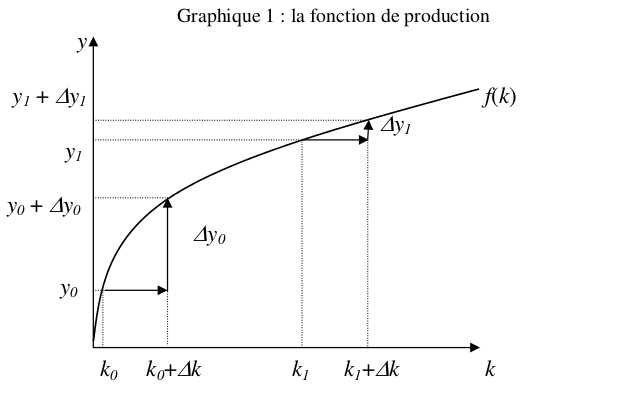
\includegraphics[width=12cm]{graph1.png}
\end{center}
La courbe passe par l'origine. Cela semble raisonnable dans la mesure où les travailleurs ne pourraient rien produire du tout sans capital. La courbe est croissante, ce qui est du à l'hypothèse que la productivité marginale du capital est constante. On constate aussi que la pente de la courbe diminue lorsque le stock de capital par travailleur augmente. Elle est \textit{concave}, ce qui vient de l'hypothèse de rendements factoriels décroissants. Une même augmentation de capital ($\Delta k$) fera plus augmenter la production si le stock de capital par travailleur initial est faible que s'il est élevé ($\Delta y_0 > \Delta y_1$). \\
On voit donc que si la technologie est donnée la fonction de production l'est aussi et la seule chose qui puisse faire augmenter le revenu par tète est une augmentation du stock de capital.
\subsection{L'accumulation de capital}
C'est l'investissement qui permet d'augmenter le capital.
\subsubsection{La répartition de la production entre investissement et consommation}
On part d'une hypothèse simple : l'épargne est simplement proportionnelle au revenu. On écrira une \textit{fonction d'épargne} de la forme :
$$ S = s.Y$$
dans laquelle $S$ représente l'épargne totale du pays et le paramètre $s$ mesure le taux d'épargne ou encore la \textit{propension à épargner}. Comme c'est un paramètre, il est indépendant de toutes les autres variables du modèle. Comme l'investissement est égal à l'épargne, on peut écrire que l'investissement est lui aussi proportionnel au revenu :
$$ I = S = s.Y $$
$$ \Rightarrow I = s.Y $$
\subsubsection{La variation du stock de capital}
Le stock de capital est un stock et les investissements sont un flux $\rightarrow$ le stock de capital est constitué des investissements passés. L'investissement d'une année vient donc s'ajouter au stock de capital initial. Mais ce n'est pas le seul mécanisme qui fait varier les stocks. Il faut aussi tenir compte du fait que, chaque année, une partie du stock de capital doit être remplacée. C'est la \textit{dépréciation du capital}. Ce phénomène décrit le fait que les machines utilisées s'usent, vieillissent et finissent par partir à la casse. La quantité de capital qui quitte le service chaque année est mesurée par les \textit{amortissements}. Pour tenir compte de ce phénomène, on va supposer qu'il se fait à un taux constant $\delta$. En d'autres termes, on va supposer que chaque année les amortissements représentent une part constante $\delta$ du capital :
$$ Am = \delta .K$$ 
On peut donc dire que l'évolution du stock de capital dépends maintenant de deux flux : les investissements et les amortissements. Les investissements font augmenter  le stock alors que les amortissements le font diminuer. \\
On peut donc dire que :
\begin{align*}
 & K_{t+1}  = K_t + I_t - Am_t \\
 \Leftrightarrow & K_{t+1}  = K_t + sY_t - \delta K_t \\
 \Leftrightarrow & K_{t+1} - K_t  = sY_t - \delta K_t \\
 \Rightarrow & \Delta K_t = sY_t - \delta K_t
\end{align*}
où $\Delta K_t$ représente la variation du stock de capital au cours de l'année $t$ qui est aussi un flux. Dans cette dernière expression nous n'avons plus que des flux. On va maintenant exprimer cette expression en terme de flux par travailleurs. On suppose que la population est constante, c'est pourquoi $L$ n'est pas suivi par un indice de temps.
\begin{align*}
  \frac{\Delta K_t}{L} & = s \frac{Y_t}{L} - \delta \frac{K_t}{L} \\
  \Rightarrow \Delta k_t & = sy_t - \delta k_t
\end{align*}
Cette expression signifie que la variation du stock de capital par tête correspond exactement à la différence entre l'investissement total par tête et l'investissement nécessaire à remplacer la fraction du stock de capital par tête qui s'est dépréciée. Puisque la production par tête est une fonction du stock de capital par tête, on peut encore simplifier ça en : 
\begin{center}
  \fbox{$\Delta k_t = sf(k_t) - \delta k_t$}
\end{center}
Il s'agit là de l'équation centrale du modèle de Solow.
\section{La croissance dans le modèle de Solow}
\subsection{L'état stationnaire}
L'\textit{état stationnaire} se définit comme l'état dans lequel plus aucune variable endogène ne varie. En particulier, le stock de capital par travailleur y reste constant. On va baptiser $\overline{k}$ la valeur stationnaire du stock de capital. On peut préciser cette valeur :
$$ \Delta \overline{k} = sf(\overline{k}) - \delta\overline{k} = 0 $$ 
\begin{center}
  $\Rightarrow$ \fbox{$sf(\overline{k}) = \delta\overline{k}$}
\end{center}
Cette expression montre que le stock de capital stationnaire est déterminé par le fait qu'il permet une production telle que l'épargne va tout juste permettre de compenser les amortissements. Comme l'investissement compense exactement les amortissements, le stock de capital reste constant. \\
Cette condition peut se traduire graphiquement de façon très simple. L'épargne étant proportionnelle au revenu, elle va se déduire de la fonction de production. L'amortissement quant à lui va être représenté par une droite passant par l'origine et dont la pente est égale à $\delta$. L'état stationnaire correspond alors à l'intersection entre la courbe qui représente l'épargne et la droite qui représente l'amortissement. \\
\begin{center}
  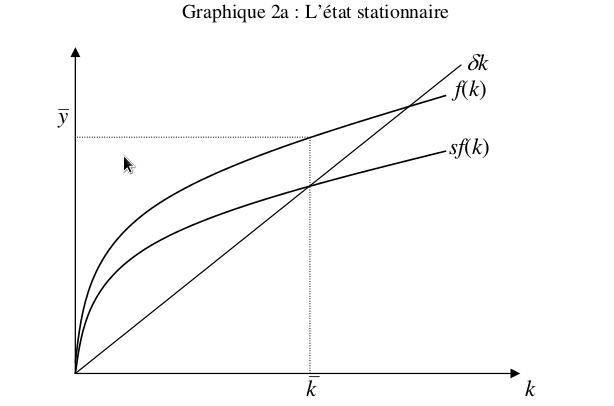
\includegraphics[width=12cm]{graph2.png}
\end{center}
Il y a donc un et un seul état stationnaire, et il correspond à une seule valeur du stock de capital par travailleur. Il y a donc aussi une seule valeur du revenu par tête. Puisque le stock de capital par tête est par définition constant à l'état stationnaire, la production par tête sera elle aussi constante. L'état stationnaire correspond donc à une situation de croissance nulle. \\
Chaque unité de capital supplémentaire augmente à la fois le revenu, donc l'épargne et l'investissement, et l'amortissement. Cependant, l'amortissement augmente proportionnellement au stock de capital alors que le revenu augmente moins que proportionnellement au stock de capital, à cause des rendements décroissants. L'amortissement finit fatalement par rattraper l'investissement.
\subsection{La convergence vers l'état stationnaire} 
\begin{center}
  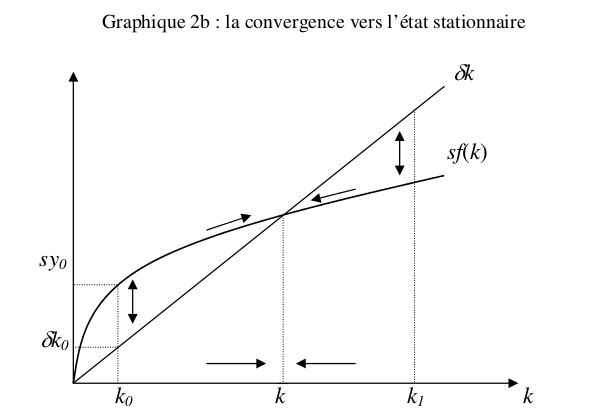
\includegraphics[width=12cm]{graph2b.png}
\end{center}
On constate qu'en $k_0$ on a $sy_0 > \delta k_0$, ce qui signifie que pendant l'année le pays va investir plus que ce qui est nécessaire pour compenser l'amortissement. Le stock de capital va donc augmenter et se rapprocher de sa valeur stationnaire $\overline{k}$ . Le même raisonnement s'applique tant que le stock de capital n'a pas atteint sa valeur stationnaire, c'est à dire à gauche du point d'intersection entre les deux courbes. Inversement,  si le pays a dépassé le stock de capital stationnaire, l'amortissement est supérieur à l'investissement, ce qui va diminuer le stock de capital et rapprocher ce dernier de son niveau stationnaire. \\
C'est la \textit{convergence} des économies. \\
Puisque plus le stock de capital est proche de sa valeur stationnaire moins l'écart entre l'épargne et l'investissement est élevé, on peut conclure que la croissance d'un pays sera d'autant plus lente que son stock de capital sera proche de son état stationnaire.
\section{La relation entre croissance et épargne}
Lorsqu'on utilise le modèle de Solow pour réfléchir à la relation entre une variable et une autre on doit se rappeler que le modèle peut connaître deux états : le premier est l'état stationnaire et le second est la convergence vers l'état stationnaire. Puisque l'économie se comporte différemment dans ces deux cas, il faut les étudier séparément.
\subsection{L'absence de relation entre épargne et croissance à l'état stationnaire}
En absence de progrès technique, la croissance est forcément nulle à l'état stationnaire. L'épargne ne peut donc pas avoir d'effet su la croissance à l'état stationnaire.
\begin{center}
  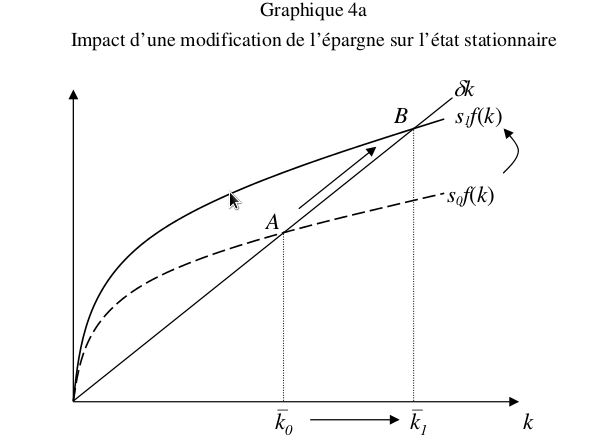
\includegraphics[width=12cm]{graph3.png}
\end{center}
Cependant, une modification de l'épargne doit bien avoir des répercussions sur l'économie. Supposons comme sur le graphique que le taux d'épargne augmente pour passer d'un niveau $s_0$ à un niveau $s_1$. Cette augmentation du taux d'épargne se traduit par un déplacement vers le haut de la courbe d'épargne. Elle coupe désormais la droite qui représente les amortissements en un nouveau point, situé au dessus et à droite du précédent. L'augmentation du taux d'épargne se traduit donc par le passage à un nouvel état stationnaire qu'on peut comparer au précédent. Par définition, le taux de croissance y est le même et est nul. En revanche, le nouveau stock de capital stationnaire est supérieur au précédent, ce qui implique que la production a aussi augmenté. On peut donc conclure que l'augmentation du taux d'épargne dans le modèle de Solow se traduit à terme par une augmentation du stock de capital et de la production par habitant. \\
Ceci a une implication pour l'hypothèse de convergence : on peut remarquer que deux économies ne convergeront vers le même revenu que si elles ont le même taux d'épargne. Si ce n'est pas le cas, elle convergeront vers des états stationnaires différents. C'est pourquoi on parle de \textit{convergence conditionnelle}. \\
La consommation n'est pas affectée de la même manière par les variations du taux d'épargne. En effet, la consommation est soumise à deux effets contradictoires : 
\begin{itemize}
  \item L'augmentation de la production augmente le revenu.
  \item Mais une part plus importante du revenu est épargnée et investie.
\end{itemize}
Par conséquent, l'effet total d'une augmentation du taux d'épargne sur la consommation est ambigu. On peut cependant prédire qu'il sera positif si le taux d'épargne initial est faible et négatif si le taux d'épargne initial est élevé. \\
On peut déterminer le taux d'épargne qui maximise la consommation, et on obtient alors la \textit{règle d'or d'accumulation du capital}.
\subsection{Une relation croissante entre épargne et croissance hors de l'état stationnaire}
Supposons qu'il existe deux économies absolument identiques et qui disposent au départ du même stock de capital $k_{initial}$ inférieur au stock stationnaire. La seule différence entre elles est leur taux d'épargne: la première connaît un taux d'épargne faible $s_0$ et la seconde a un taux d'épargne élevé $s_1$. 
\begin{center}
  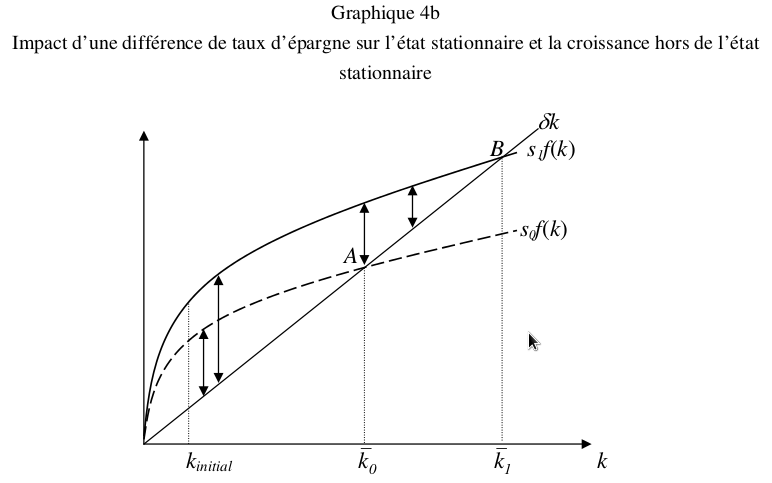
\includegraphics[width=12cm]{graph4.png}
\end{center}
Ce graphique permet de voir que l'économie qui épargne le moins sera aussi celle qui accumulera du capital le moins vite. Hors de l'état stationnaire il existe une relation positive entre le taux d'épargne et le taux de croissance. \\
On peut utiliser aussi ce graphique pour analyser la transition entre un état stationnaire à épargne faible et un nouvel état stationnaire lorsque le taux d'épargne a augmenté (passage du point $A$ au point $B$). On voit que lorsque le taux d'épargne augmente l'investissement devient instantanément plus élevé que l'amortissement. Le stock de capital se met donc à augmenter. Cependant, au fur et à mesure que le stock de capital augmente, la productivité marginale du capital diminue, et l'accumulation du capital se ralentit. Après un saut initial, le taux de croissance diminue pour tendre vers 0 lorsque l'économie se rapproche de son état stationnaire. Ceci peut être résumé par le graphique suivant : 
\begin{center}
  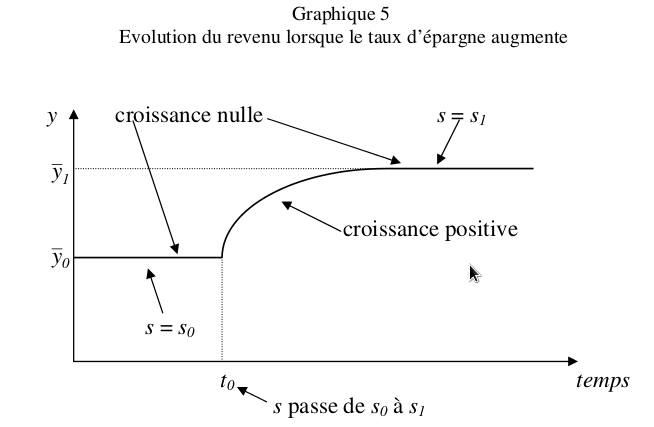
\includegraphics[width=12cm]{graph5.png}
\end{center}
On peut donc conclure qu'une augmentation définitive du taux d'épargne ne provoque qu'une croissance temporaire.

\chapter{Le rôle du progrès technique dans la croissance}
\section{Introduction : Les origines}
On peut résumer le progrès en le définissant comme tout ce qui permet d'améliorer le bien-être des consommateurs. Le progrès a donc à la fois une dimension quantitative et une dimension qualitative.
\section{Une mesure de la part du progrès dans la croissance}
\subsection{Construction du résidu de Solow}
On prends à présent compte du progrès technique en écrivant :
$$ Y = A F(K,L) $$
où $A$ reprrésente le progrès technique. L'idée est ici que le progrès vient augmenter la productivité des autres facteurs de production. On appelle ce paramètre la \textit{productivité globale des facteurs} ou \textit{productivité totale des facteurs} (PTF). C'est cette PTF qu'on cherche à mesurer. \\
La méthode proposée par Solow pour mesurer la croissance de la PTF repose sur la fonction de production et l'hypothèse de rendements d'échelle constants. Le principe en est très simple. Supposons que sur une période donnée le stock de capital et la population active aient augmenté dans la meme proportion, par exemple $1\%$. En raison des rendements d'échelle constants, la production devrait avoir également augmenté de $1\%$. Supposons que sur la même période le taux de croissance observé ait en fait été de $2\%$. Cela signifie que les variations du stock de capital et de la population active ne permettent pas d'expliquer la totalité de la croissance, puisqu'ils ne peuvent être responsables que d'$1\%$ de la croissance. Il reste un point de croissance résiduel qui n'est pas expliqué. \\
Si on reprend la fonction de production, ce point de croissance supplémentaire ne peut être dû qu'à une seule chose : une augmentation de la productivité. On mesure donc la part de la productivité dans la croissance en lui attribuant toute la croissance que l'évolution des autres facteurs de production ne peut expliquer. Voilà pourquoi on parle autant de \textit{résidu de Solow} que de la \textit{croissance de la productivité totale des facteurs}. \\
Le problème est que les quantités de facteurs de production ne croissent en général pas dans les mêmes proportions. Les facteurs ne contribuent donc pas dans les mêmes proportions à la croissance et il faut attribuer à chacun la part de croissance qui lui revient. On a donc besoin de connaitre sa \textit{productivité marginale}. \\
On va alors supposer que l'économie est parfaitement concurrentielle. A partir de cette hypothèse, on peut montrer que le taux de croissance peut être décomposé pour donner l'\textit{équation fondamentale de décomposition de la croissance} : 
\begin{center}
  \fbox{$g_y = \alpha_K g_K + (1-\alpha_K) g_L + g_{PTF}$} 
\end{center}
dans laquelle $g_y$, $g_L$, $g_K$ et $g_{PTF}$ représentent respectivement les taux de croissance du revenu, de la population active, du stock de capital et de la productivité totale des facteurs. Ils sont tous exprimés en pour-cents. \\
Le coefficient $\alpha_K$ est compris entre 0 et 1 et mesure la part du capital dans le revenu, c'est à dire $\frac{rK}{Y}$ où $r$ est la rémunération du capital. $(1-\alpha_K)$ mesure donc la partie du travail dans le revenu. On estime en général que $\alpha_K$ est environ égal à $0.3$ et donc $(1-\alpha_K)$ à $0.7$. Or ces parts sont observables, tout comme $g_y$, $g_L$ et $g_K$, ce qui signifie qu'on peut déduire la croissance de la productivité à partir de l'équation précédente : 
\begin{center}
  \fbox{$g_{PTF} = g_y - \alpha_K g_K - (1-\alpha_K) g_L \equiv Residu$} 
\end{center}
C'est cette équation fondamentale qui permet de déduire la part du progrès technique dans la croissance ou résidu de Solow. L'expression de résidu est préférable aux autre parce qu'il s'agit bien de la part de la croissance qu'on ne parvient pas à expliquer.
\subsection{La part du progrès technique dans la croissance}
On peut utiliser le résidu pour mesurer et comparer la part du progrès technique dans la croissance de plusieurs pays. On peut observer que : 
\begin{itemize}
  \item Le progrès technique est responsable d'une part très importante de la croissance.
  \item La convergence des productions par travailleur est largement due au fait que les économies initialement plus pauvres connaissent un taux de croissance de leur productivité plus rapide. Ici encore l'accumulation de capital ne joue qu'un rôle secondaire.
\end{itemize}
\section{Le progrès technique dans le modèle de Solow}
\subsection{Effet d'une croissance ponctuelle de la productivité}
Supposons qu'une innovation quelconque vienne augmenter la productivité des facteurs de production. Cette innovation signifie qu'on va pouvoir produire plus avec la même quantité de facteurs de production. Dans le cadre du modèle de Solow, on peut représenter cet évènement en supposant qu'une nouvelle fonction de production remplace l'ancienne et augmente la production pour chaque valeur du stock de capital par travailleur : 
\begin{center}
  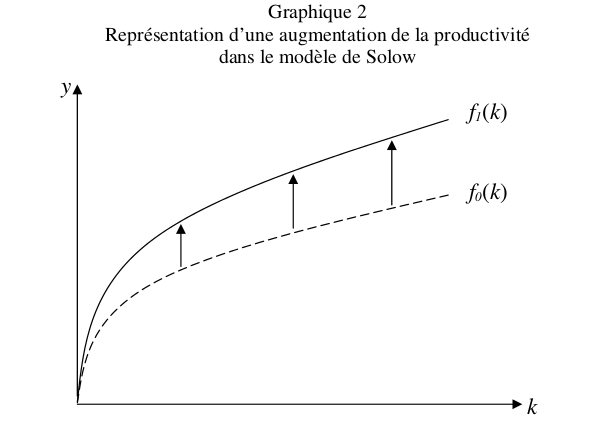
\includegraphics[width=12cm]{graph6.png}
\end{center}
La déformation de la fonction de production va affecter la fonction d'épargne. On peut alors déterminer l'effet des gains de productivité sur l'état stationnaire : 
\begin{center}
  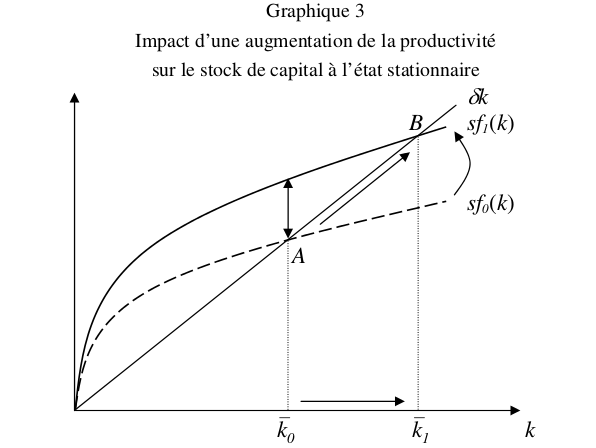
\includegraphics[width=12cm]{graph7.png}
\end{center}
L'épargne par travailleur est à présent systématiquement supérieure à ce qu'elle était auparavant pour un même stock de capital. Cela implique l'état stationnaire se modifie (passage du point $A$ au point $B$). On constate que le stock de capital par travailleur a augmenté grâce à l'augmentation de la productivité.
\begin{center}
  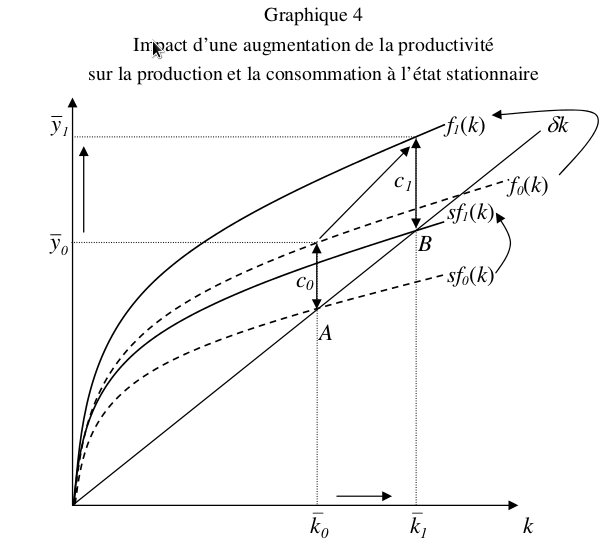
\includegraphics[width=12cm]{graph8.png}
\end{center}
L'augmentation du stock de capital n'est pas sans effet sur la production. En effet, puisque la productivité et le stock de capital ont augmenté, on peut déduire que la production par travailleur a elle aussi augmenté. La nouvelle valeur stationnaire du revenu est bien supérieure à ce qu'elle était avant. De plus, la consommation par travailleur augmente sans ambiguïté, puisque le revenu par travailleur augmente alors que la propension à épargner reste constante. \\
On peut donc conclure que les gains de productivité permettent de faire augmenter le stock de capital, la production et la consommation par travailleur, même lorsque l'état stationnaire est atteint. Ce résultat ne concerne cependant qu'une augmentation ponctuelle de la productivité.
\subsection{La prise en compte d'un augmentation tendancielle de la productivité}
Pour intégrer le progrès technique de façon systématique, il faut modifier la fonction de production agrégée pour y faire apparaître un paramètre de productivité. Il y aurait plusieurs façons de le faire mais Solow choisit la suivante :
$$Y = F(K,AL)$$
Désormais, le paramètre qui mesure la productivité n'affecte plus à présent que le travail. \\
L'hypothèse que le progrès affecte la productivité du travail peut s'interpréter de deux façons équivalentes : 
\begin{itemize}
  \item Elle signifie que le progrès technique réduit le nombre de travailleurs nécessaires pour produire une quantité donnée. Si $A$ double, il faudra deux fois moins de travailleurs pour produire la même chose.
  \item Elle signifie aussi que le progrès augmente la production des travailleurs. Le doublement de $A$ a alors le même effet sur la production totale qu'un doublement de la population active. Pour tenir compte de ce phénomène, on appelle $AL$ la \textit{quantité de travail effectif}.
\end{itemize}
Pour tenir compte de l'augmentation continue de la productivité, Solow suppose que le paramètre $A$ augmente à taux constant $g_A$. Ce taux est exogène, il n'est donc pas expliqué et fait partie des hypothèse du modèle. La conséquence de cette hypothèse est que la fonction de production se déforme en permanence. Cela implique que le stock de capital par travailleur et la production par travailleur augmentent en permanence. \\
On peut même calculer leur taux de croissance à l'état stationnaire. On peut montrer que le taux de croissance du stock de capital est le même que celui de la production par tête, et qu'ils correspondent tous les deux au taux de croissance de la productivité $g_A$. \\
Ainsi, le modèle de Solow est compatible avec une croissance soutenue de la production par travailleur, même à l'état stationnaire. En revanche, la croissance à l'état stationnaire n'est pas expliquée par le modèle. \\
En dehors des périodes transitoires ou le taux d'épargne joue un rôle, les différences de taux de croissance du revenu par habitant dépendent uniquement du taux de croissance de la productivité. Cette conclusion est également applicable aux différences entre les pays : si un pays croit durablement plus vite qu'un autre, c'est que sa productivité croit plus vite.
\section{Les déterminants du progrès technique}
\subsection{L'investissement dans la recherche}
\subsubsection{Motivation des investissements en R\&D}
Pour Schumpeter, l'innovation est une activité économique qui a pour objet la recherche du profit. C'est parce que les \textit{entrepreneurs} espèrent augmenter leur profit qu'ils investissent des ressources dans la production de connaissances nouvelles. Ces connaissances nouvelles vont déboucher sur des produits nouveaux et des procédés nouveaux. Ces derniers vont conférer à leur inventeur une position de monopole grâce à laquelle les entrepreneurs vont pouvoir obtenir des profits de monopole au lieu d'un produit nul sur un marché concurrentiel. C'est pour obtenir une telle rente de monopole que les entrepreneurs consacrent des ressources à la R\&D. Cependant, la rente de monopole n'est pas éternelle et finit par s'éroder à cause de la réaction des concurrents. \\
La conséquence de cette érosion des rentes dues à l'innovation passée est que les entreprises ne peuvent se contenter d'avoir innové une fois pour toutes mais doivent constamment continuer d'investir dans la R\&D. La concurrence pour les rentes de monopoles engendre donc une tendance continue à l'innovation qui se traduit par une augmentation de la productivité.
\subsection{L'efficacité des efforts de recherche}
\subsubsection{Facteurs institutionnels}
La fécondité du processus de recherche se définit comme la façon dont les investissements en R\&D vont se traduire par des innovations. Deux pays qui investissent des sommes comparables dans la recherche pourront obtenir des résultats en termes de croissance très différents en fonction de la fécondité de leurs système de recherche. \\
La fécondité de la recherche mesure en quelque sorte le rendement des investissements en R\&D. Il y a cependant une différence importante entre le rendement d'un investissement en R\&D et celui des investissement en capital physique : le rendement des investissement physiques est en général connu avec certitude ou avec peu d'aléas. \\
A l'échelle d'un pays c'est principalement l'organisation de la recherche qui va déterminer sa fécondité. En particulier, la relation entre la recherche fondamentale et la recherche appliquée est cruciale. La première développe des théories plus générales et parfois abstraites alors que la seconde utilise ces résultats pour développer de nouveaux usages. Ces deux branches de la recherche sont indissociables. \\
La relation entre les deux est difficile à cerner et le dosage optimal est donc une question en débat. Un facteur institutionnel fondamental est la participation de l'état dans la recherche. L'état joue en effet un rôle important non seulement en accordant des brevets mais aussi en participant directement à l'effort de recherche.\\
Il faut alors déterminer le volume de l'intervention de l'état dans l'effort de recherche et déterminer quel type de recherche il doit financer. L'idée est alors de financer les activités qui ne seraient pas entreprises par le secteur privé en l'absence de financement public. Cet argument suggère que l'état prenne en charge au moins la recherche fondamentale dont les applications à court terme sont rares.
\subsubsection{Le caractère cumulatif des connaissances}
Cela signifie que toute innovation s'appuie sur les connaissances disponibles, et donc sur les innovations passées. Parfois une innovation ne consiste que dans l'idée de rapprocher deux techniques ou produits existants. \\
Le caractère cumulatif des connaissances a des implications de première importance pour la dynamique des économies. Il implique en effet qu'une économie pourra innover d'autant plus qu'elle disposera déjà d'un stock de connaissances important. Si on suppose que le stock de connaissances détermine la productivité, cela signifie qu'une économie initialement plus productive verra sa productivité croître plus rapidement que les autres.\\
Une économie plus riche au départ croîtra plus vite que les autres $\Rightarrow$ on aura un phénomène de divergence. \\
Cette intuition se trouve à la base des théories de la croissance développées à la fin des 80's et au début des 90's qui ont été baptisées \textit{théories de la croissance endogène}. Ces dernières reposent sur des mécanismes par lesquels la croissance de la productivité est d'autant plus rapide que le revenu est élevé au départ. Ces mécanismes reposent notamment sur l'incitation à innover ou l'apprentissage par la pratique, c'est à dire le fai qu'un travailleur accumulera d'autant plus d'expérience qu'il aura produit beaucoup. \\
Ces modèles proposent une explication cohérente au fait que les pays pauvres ne convergent pas vers les niveaux de revenu des pays riches. Cette explication peut se résumer par le graphique suivant :
\begin{center}
  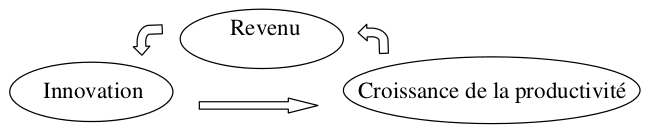
\includegraphics[width=12cm]{graph9.png}
\end{center}
Les pays riches bénéficient d'un cercle vertueux. Comme leur revenu est élevé au départ, ils innonvent beaucoup. Comme ils innovent beaucoup, leur productivité augmente rapidement, ce qui augmente leur revenu, ce qui augmentera la vitesse d'innovation, etc. Les pays pauvres au contraire sont enfermés dans le cercle vicieux inverse. Ce cercle vicieux est ce qu'on appelle la \textit{trappe à pauvreté}.

\part{L'économie dans le court terme : les fluctuations}
\chapter*{Introduction}
Dans la partie précédente on a supposé que l'économie connaissait un taux de croissance constant sur de longues périodes. On a proposé des explications au fait que certaines économies connaissaient une croissance moyenne forte alors que d'autres stagnaient. Pourtant, même les économies les plus performantes connaissent des périodes de croissance plus ou moins rapide. On observe en effet des écarts réguliers par rapport à la tendance. On appelle \textit{fluctuations} ces variations de la croissance autour de sa tendance de long terme. \\
On a longtemps utilisé le terme de \textit{cycle} mais celui-ci suggère une parfaite régularité des variations de la croissance à court et moyen terme. Le terme de \textit{crise} est aussi employé mais il désigne une phase du cycle et a une connotation pathologique.
\begin{center}
  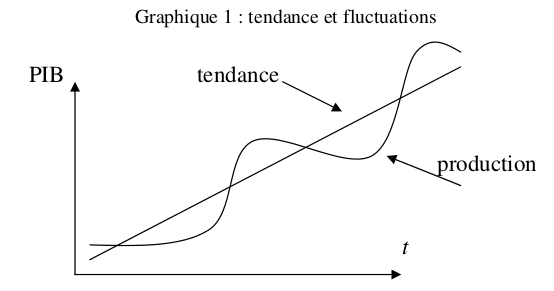
\includegraphics[width=12cm]{graph10.png}
\end{center}
Sur un horizon de quelques années, le taux de croissance est beaucoup plus instable que ce que laisseraient supposer les modèles de croissance. L'analyse des fluctuations consiste donc à chercher à expliquer la succession de phases d'expansion et de récession. On peut se demander s'il faut pour cela construire des théories spécifiques ou essayer de raffiner les théories déjà vues. Certains économistes considèrent qu'il est possible d'expliquer les fluctuations en restant dans le cadre concurrentiel que nous avons déjà utilisé. Selon eux, il vaudrait mieux prendre en compte les décisions inter-temporelles et les délais d'ajustement qui apparaissent dans la gestion de la production et de l'investissement. \\
Pourtant, il existe au moins deux différences importantes entre le court et le long terme : 
\begin{itemize}
  \item A court terme les prix sont rigides.
  \item A court terme on constate également que la production peut être inférieure à son niveau potentiel. Les récessions ne sont pas dues à une réduction des capacités de production de l'économie mais à une utilisation moins intensive de ces capacités de production.
\end{itemize}
On a développé une mesure de l'utilisation du potentiel productif d'une économie appelée \textit{taux d'utilisation des capacités} (\textit{TUC}). On constate que le TUC peut fluctuer de manière significative.
\chapter{Le marché des biens}
\section{Introduction : L'importance de la demande de biens}
Précédemment, on a décrit l'évolution de l'économie en se concentrant sur l'offre de biens et en négligeant les effets de la demande. Puisque c'était un raisonnement à long terme c'était l'évolution des capacités de production qui déterminait l'évolution de la production et on pouvait supposer que la demande absorbait forcément ce qui était produit. \\
Si on veut s'intéresser au court terme,  et donc à la possibilité de surproduction, il faut intégrer la demande de biens dans le raisonnement. Il est en effet nécessaire de comprendre pourquoi la demande de biens peut être insuffisante pour absorber la production. \\
\section{Les composantes de la demande}
Le raisonnement se place ici pour l'instant dans le cadre d'une économie fermée. La demande globale a donc trois composantes : la consommation, l'investissement et les dépenses publiques.
\subsection{La consommation}
On entends souvent dire que la consommation est le ``moteur de la croissance''. Cette expression repose implicitement sur une vision keynésienne du fonctionnement de l'économie.
\subsubsection{La consommation : une fonction du revenu courant}
Le pilier de cette analyse sera la fonction de consommation keynésienne donc Keynes n'a pas donné de définition algébrique mais fonde son raisonnement sur une \textit{loi psychologique fondamentale} qui a été interprétée et formalisée par la suite. Cette loi exprime que ``en moyenne et la plupart du temps, les hommes tendent à accroître leur consommation à mesure que leur revenu croit, mais non d'une quantité aussi grande que l'accroissement du revenu''. \\
Par commodité, on va retenir une forme très simple de la fonction de consommation et vérifier si elle peut correspondre à l'idée de Keynes. La fonction de consommation la plus simple est linéaire : 
\begin{center}
  \fbox{$C = c.Y + C_0$} 
\end{center}
où 
\begin{itemize}
  \item $c$ est appelé la \textit{propension marginale à consommer} ($PmC$). Ce paramètre mesure l'augmentation de la consommation provoquée par une augmentation du revenu d'une unité La propension marginale à consommer est définir de façon générale comme la dérivée de la fonction de consommation par rapport au revenu :
$$ PmC = \frac{\partial C}{\partial Y} = c $$
    \item $C_0$ mesure la consommation qui serait observée si le revenu était nul. On l'appelle donc la \textit{consommation incompressible}. 
\end{itemize}
D'après la loi psychologique fondamentale, la consommation doit augmenter avec le revenu, ce qui signifie que la $PmC$ doit être positive $\rightarrow$ $c>0$. Et puisque cette augmentation n'est pas aussi grande que l'accroissement du revenu, $0 < c < 1$. On considère en général qu'une valeur réaliste de $c$ tourne autour de $0.8$. \\
On définit aussi la \textit{propension moyenne à consommer} ($PMC$) qui est la part du revenu qui est consacrée à la consommation :
$$ PMC \equiv \frac{C}{Y} = c + \frac{C_0}{Y} $$
On constate alors que la propension moyenne à consommer est une fonction décroissante du revenu. \\
La représentation graphique de cette fonction de consommation est très simple. Il s'agit d'une droite de pente $c$ et d'origine $C_0$ :
\begin{center}
  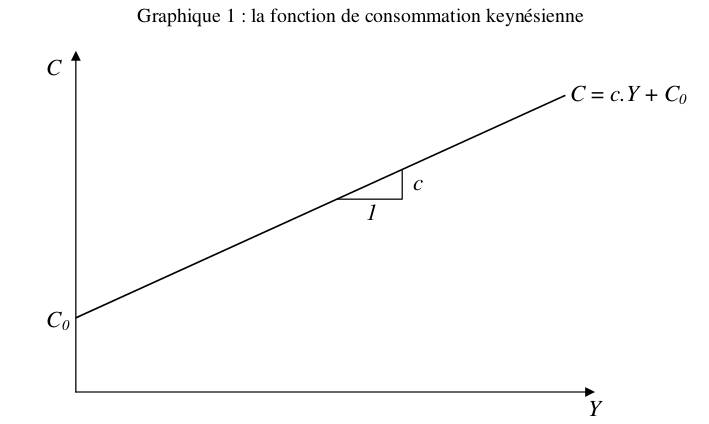
\includegraphics[width=12cm]{graph11.png}
\end{center}
La décision de consommer est la contrepartie de la décision d'épargner. On peut donc déduire la fonction d'épargne de la fonction de consommation : 
\begin{align*}
  S & \equiv Y - C = Y - (c.Y + C_0) \\
  \Rightarrow S & = (1 - c) Y - C_0
\end{align*}
On constate que l'épargne ne dépends que tu revenu courant. Tout se passe comme si l'épargne n'était que ce qui restait après la consommation. Les consommateurs ne tiennent ainsi pas compte de l'évolution à venir de leur revenu. Ceci a été vite critiqué.
\subsubsection{La consommation : une fonction des revenus futurs}
On reproche à Keynes d'avoir créé une fonction de consommation pour servir son raisonnement sans avoir utilisé de fondements micro-économiques. Or l'analyse micro-économique montre que la décision de consommer reposer sur un arbitrage entre consommation présente et future. Lorsqu'ils font cet arbitrage, les consommateurs tiennent compte de leur contrainte budgétaire inter-temporelle. Par conséquent, la consommation devrait dépendre non seulement du revenu courant, mais aussi de tous les revenus futurs et du taux d'intérêt. \\
L'effet du taux d'intérêt sur la consommation est ambigu d'un point de vue théorique et difficile à mettre en évidence empiriquement. Cela vient du fait que l'effet de revenu et l'effet de substitution d'une variation du taux d'intérêt ont tendance à se compenser. \\
Par exemple, considérons un agent qui est un préteur net et qui constate une diminution du taux d'intérêt. Comme le taux d'intérêt a baissé, le rendement de l'épargne s'est également réduit, ce qui incite notre agent à épargner moins qu'auparavant et donc à consommer d'avantage. C'est l'effet de substitution. Mais la diminution de la rémunération de l'épargne réduit le revenu des prêteurs et notre agent se retrouve donc moins riche qu'auparavant. Il sera donc incité à réduire sa consommation. C'est l'effet de revenu. Les deux effets s'opposent donc bien. L'effet total d'une variation du taux d'intérêt est donc indéterminé et probablement d'une ampleur limitée. Par conséquent, on négligera cet effet et on supposera que la consommation est indépendante du taux d'intérêt. \\
En revanche, le rôle des revenus futurs à été reconnu et les raisonnements proposés à ce propos reposent sur l'hypothèse que les consommateurs sont prévoyants et que par conséquent ils ne peuvent déterminer leur consommation sans tenir compte de l'évolution de leurs revenus. \\
Friedman argue que si le consommateur est prévoyant, il ne fondera pas ses décisions de consommer sur son revenu courant, qui peut être très variable, mais sur l'évolution prévisible de son revenu. Plus précisément, il convient de distinguer le \textit{revenu permanent} ($Y^P$) et le \textit{revenu transitoire} ($Y^T$). LE revenu permanent est en quelque sorte le revenu que le consommateur peut anticiper en moyenne. Le revenu transitoire est un revenu accidentel, par exemple un gain à la loterie ou des heures supplémentaires dues à une relance temporaire de l'activité. Le revenu courant est la somme de ces deux revenus : $Y = Y^P + Y^T$. Ce dernier peut parfois être inférieur au revenu permanent, par exemple pendant une période de récession transitoire. \\
Dans tous les cas, si le consommateur est prévoyant il basera sa consommation sur son revenu permanent. S'il bénéficie d'un revenu courant supérieur à son revenu permanent ($Y^T > 0$) il épargnera d'avantage. Si le revenu courant est inférieur au revenu permanent ($Y^T < 0$), il empruntera ou puisera dans son épargne. Par conséquent, la seule relation stable qui existe est celle qui relie la consommation au revenu permanent : $C = k.Y^P$. La relation entre le revenu transitoire et la consommation doit être nulle ou très faible. \textit{L'hypothèse du revenu permanent} suggère donc que la fonction de consommation keynésienne est mal spécifiée. \\
Modigliano va plus loin en faisant remarque que l'évolution du revenu au cours de la vie est largement prévisible : on commence à 0, puis les revenus augmentent avec l'âge et l'expérience, puis les revenus redeviennent nuls à la retraite et il faut puiser dans son épargne pour continuer à consommer. Si le consommateur est prévoyant et veut maintenir une consommation à peu près constante, il tiendra compte de l'évolution de son épargne au cours de sa vie. C'est la base de \textit{l'hypothèse du cycle de vie}. On peut alors d'écrire l'évolution de l'épargne et du patrimoine :
\begin{center}
  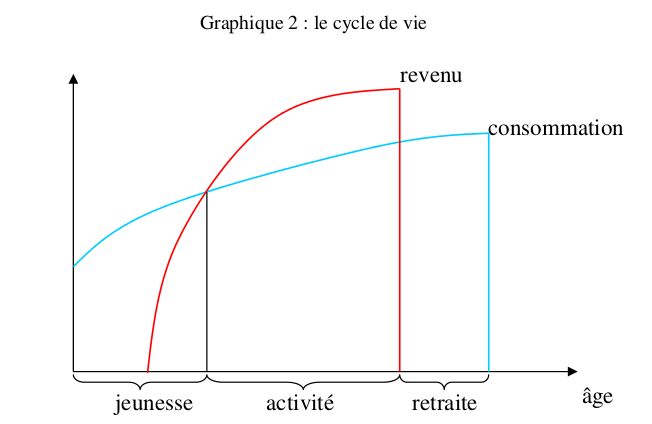
\includegraphics[width=12cm]{graph12.png}
\end{center}
Au cours de sa jeunesse le consommateur a un revenu très faible et va donc emprunter ou puiser dans son patrimoine. Lorsqu'il se met à travailler son revenu augmente et il finit par pouvoir couvrir sa consommation courante et rembourses dettes et constituer une épargne. Lorsqu'il part à la retraite, le consommateur va puiser dans son épargne pour maintenir sa consommation jusqu'à son décès. \\
Cette théorie a deux implications essentielles au niveau agrégé : 
\begin{itemize}
  \item Elle suggère qu'il existe une relation entre la structure démographique d'un pays et son taux d'épargne : les pays très jeunes ou très vieux auront tendance à moins épargner.
  \item Elle suggère que les fluctuations du revenu de court terme n'ont qu'une importance secondaire dans la détermination de la consommation.
\end{itemize}
Il existe donc des arguments forts pour remettre en cause la relation entre revenu courant et consommation courante, mais cette relation reste cependant à la base de beaucoup de théories macroéconomiques pour plusieurs raisons : 
\begin{itemize}
  \item Lorsqu'on considère qu'un consommateur n'est contraint que par une contrainte budgétaire inter-temporelle qui n'est que la somme actualisée de ses revenus futurs, on fait implicitement l'hypothèse qu'il a un accès illimité au crédit. Or le marché du crédit ne fonctionne pas de façon parfaite. On dit que certains consommateurs sont \textit{rationnés} et qu'ils subissent alors une \textit{contrainte de liquidités}. Lorsqu'un consommateur est rationné, sa consommation dépends principalement de son revenu courant et on retrouve alors des comportements compatibles avec la fonction de consommation keynésienne.
  \item Tant la théorie du revenu permanent que la théorie du cycle de vie amènent à distinguer les variations temporaires et permanentes du revenu.
\end{itemize}
Tout ceci nous amène à considérer que la fonction de consommation keynésienne qui implique que la propension moyenne à consommer diminue avec le revenu est une approximation convenable pour étudier les fluctuations temporaires du revenu.
\subsection{L'investissement}
L'investissement est un des agrégats les plus variables. Compte tenu de sa part dans le PIB, on doit s'(attendre à ce qu'il soit à l'origine d'une partie des fluctuations conjoncturelles.
\subsubsection{L'investissement : une fonction du taux d'intérêt}
La microéconomie nous apprend que le \textit{coût d'opportunité} de l'investissement est constitué par le taux d'intérêt des titres. Lorsqu'on détermine l'équilibre du producteur, on montre que le stock de capital de l'entreprise va être déterminé de façon à ce que la productivité marginale du capital soit égale au taux d'intérêt,  c'est à dire au rendement de l'obligation. Comme la productivité marginale du capital est décroissante, la quantité de capital utilisée va être une fonction décroissante du taux d'intérêt. L'investissement sera donc lui aussi une fonction décroissante du taux d'intérêt. \\
Il existe une autre raison pour laquelle l'investissement dépends du taux d'intérêt : le \textit{canal du crédit}. Le canal du crédit apparaît en situation de \textit{rationnement du crédit}, c'est à dire dans une situation ou les banques ne satisfont pas l'ensemble des demandes de prêts qui leur sont adressées Cela signifie donc que les entreprises ne pourront pas financer tous les investissements qu'elles souhaitent réaliser. Or le taux d'intérêt représente pour les banques le coût marginal des prêts. Si le taux d'intérêt augmente, les banques réduiront encore leur offre de prêts. Elles empêcheront donc davantage d'entreprises de financer leurs investissements. Le canal du crédit renforce donc l'impact négatif du taux d'intérêt sur l'investissement.
\subsubsection{L'investissement : une fonction de la demande et des anticipations}
Une entreprise investit pour augmenter ses capacités de production. quel que soit le taux d'intérêt, il ne lui sert à rien d'augmenter son stock de capital si elle ne parvient pas à écouler sa production. \\
En revanche, si la demande augmente et que l'entreprise n'est pas capable de la satisfaire, elle laissera passer des occasions d'augmenter ses profits. On voit donc que l'investissement va être une fonction croissante de la demande de biens. A l'échelle macroéconomique, la demande de biens dépend du revenu et donc de la production. On pourra donc supposer que l'investissement est une fonction de la production. \\
Enfin, lorsqu'une entreprise investit, elle acquiert du capital qu'elle pourra utiliser pendant plusieurs années. Elle doit donc tenir compte de l'effet de ce capital non seulement sur ses profits courants mais sur ses profits à venir. L'investissement va donc être une fonction des profits anticipés par l'entreprise. Ces profits anticipés dépendent à leur tour de l'évolution anticipée de la demande, des taux d'intérêt, du prix des inputs, ... mais aussi de l'optimisme des investisseurs.
 \\
En résumé, l'investissement est donc une fonction décroissante du taux d'intérêt, et croissante du revenu et des profits anticipés :
$$ I = I\left(\overset{-}{r}, \overset{+}{Y}, \overset{+}{profits^e}\right)$$
\subsection{Les dépenses de l'état}
Dans une économie fermée les dépenses publiques constituent la dernière composante de la demande et son quantitativement importantes. C'est cette composante qui peut être utilisées par le gouvernement à des fins de politique économique. Le niveau des dépenses et des prélèvements publics est en effet un choix politique même s'il doit respecter certaines contraintes. Dans tous les cas les gouvernements doivent en principe respecter leur contrainte budgétaire inter-temporelle s'ils ne veulent pas se retrouver en situation de devoir faire défaut sur leur dette. On ne tiendra pas explicitement compte de ces contraintes dans nos raisonnements, mais il faudra les garder à l'esprit pour comprendre pourquoi on ne peut pas augmenter indéfiniment le déficit ou la dette. \\
Pour l'instant on se contentera de supposer que les dépenses publiques et les impôts sont choisis librement par le gouvernement et constituent donc des paramètres du modèle.
\section{L'équilibre sur le marché des biens}
Le diagramme à 45 degrés décrit l'équilibre sur le marché des biens. Il peut etre considféré comme le premier modèle d'inspiration keynésienne.
\subsection{Le diagramme à 45 degrés}
Ce diagramme repose sur l'égalité entre l'offre et la demande sur lamrché des biens. Cependant, cette égtalité est obtenue de facon très différente de celle qui est supposée par la  microéconomie. En effet, le diagramme repose sur l'hypothèse que les prix sont fixes et que l'économie se trouven en situation de sous emploi. Cela implique que l'ajustement de l'offre et de la demande ne passe pas par l'ajustement des prix mais par celui des quantités produites. \\
En situation de sous-emploi, il existe par définition des capacités excédentaires. Les producteurs pourraient donc augmenter facilement leur production s'ils pouvaient l'écouler. Ils sont cependant contraints par la demande qui est insuffisante. On dit que la demande constitue le \textit{coté court} du marché. Dans ces circonstances, c'est la demande qui va déterminer la production. C'est pourquoi on peut étudier l'équilibre de l'économie sans décrire les conditioons de production ni définir de fonction d'offre. \\
La demande globale corresponds à la somme de la consommation, de l'investissement et des dépenses publiques. On peut donc écrire :
$$ D^G = C + I + G$$
Parmi ces trois composantes, deux sont déterminées hors du marché des biens. On négligera en effet pour l'instant le rôle des anticipations. Par ailleurs, comme l'économie est en situation de surcapacité les entreprises pourront augmenter leur production sans avoir besoin d'augmenter leurs capacités de production. \\
L'investissement dépend alors surtout du taux d'intéret qui est déterminé sur le marché financier et est donc exogène au modèle. Par conséquent, l'investissement peut être considéré comme une constante : $I = I_0$. \\
De même, les dépenses publiques sont déterminées par le gouvernement. Elles sont donc elles aussi un paramètre du modèle : $G = G_0$. \\
Par conséquent, la seule composante de la demande qui soit endogène est la consommation. On suppose qu'elle est décrite par une fonction de consommation keynésienne : $C = c.Y + C_0$. \\
On peut alors réécrire la demande globale :
$$ D^G = c.Y + C_0 + I_0 + G_0 $$
On peut alors représenter la demande globale en fonction du revenu de façon très simple :
\begin{center}
  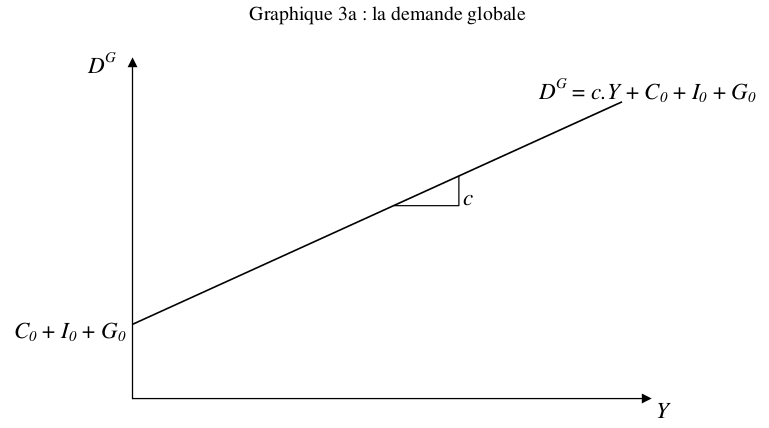
\includegraphics[width=12cm]{graph13.png}
\end{center}
La demande est donc représentée par une droite croissante dont l'ordonnée à l'origine est égale à la somme de l'investissement, des dépenses publiques et de la consommation incompressible, et la pente à la propoension marginale à consommer. Cette pente est donc inférieure à 1. \\
L'équilibre sur le marché des biens sera atteint lorsque l'offre sera tout juste égale à la demande. Au niveau agrégé, l'offre de biens est égale à la production : $Y^S = Y$. Cette équation correspond à une droite passant par l'origine et de pente égale à 1. si on utilise la même échelle en abscisse et en ordonnée, cette droite correspondra à la première bissectrice du repère et formera un angle de 45 degrés avec les deux axes, d'où le fait qu'on parle de diagramme à 45 degrés. \\
Une fois que l'offre est représentée sur le graphique, on détermine facilement l'équilibre sur le marché des biens. Il correspond à l'intersection entre la courbe de demande et la première bissectrice qui correspond à la courbe d'offre :
\begin{center}
  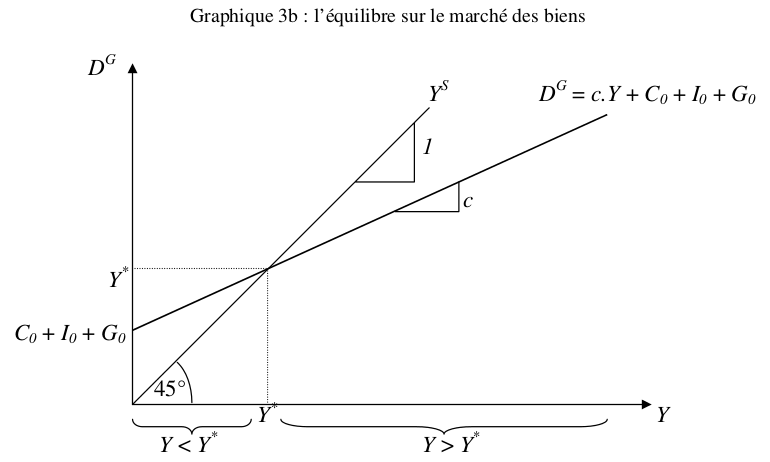
\includegraphics[width=12cm]{graph14.png}
\end{center}
Les deux courbes vont forcément se couper, il y a donc forcément un équilibre. Le revenu d'équilibre $Y^*$ peut se mesurer autant abscisse qu'en ordonnée. \\
Si les producteurs avaient surestimé la demande globale, et produit une quantité de biens supérieur à $Y^*$, les stocks vont augmenter, les producteurs vont réduire leur production et ca les rapprochera de l'équilibre. Dans le cas contraire, un raisonnement similaire les rapprochera aussi de l'équilibre. \\
On peut alors faire plusieures remarques : 
\begin{itemize}
  \item L'équilibre sur le marché des biens est stable.
  \item L'ajustement à très court terme est assuré par les variations de stocks.
  \item Il n'existe aucun mécanisme qui permette d'affirmer que le revenu d'équilibre correspond au revenu de plein emploi. Par conséquent, si pour une raison quelqconque la demande ne permet pas le plein emploi l'économie restera durablement en situation de sous emploi.
\end{itemize}
Cette dernière remarque est un premier résultat fondamental de l'analyse keynésienne. \\
Jusqu'à présent on a eu recours à un raisonnement graphique. On peut aussi écrire la condition d'équilibre sur le marché des biens et la résoudre pour déterminer le niveau d'équilibre du revenu de manière algébrique : 
\begin{align*}
  Y^S & = D^G \\
  Y & = c.Y + C_0 + I_0 + G_0 \\
  Y & - c.Y = C_0 + I_0 + G_0 
\end{align*}
\begin{center}
  $\Rightarrow$ \fbox{$Y^* = \frac{C_0 + I_0 + G_0}{1 - c}$}
\end{center}
Le revenu d'équilibre est égal à la somme des dépenses exogènes au marché des biens divisé par la propension marginale à épargner ($s = 1 - c$).
\subsection{Le multiplicateur}
L'expression du revenu d'équilibre montre que le revenu est une fonction croissante des dépenses. Par conséquent, l'augmentation de l'une des composantes de la demande se traduirait par une augmentation du revenu d'équilibre. Le multiplicateur permet de mesurer le rapport entre la variation du revenu et la variation des dépenses qui l'a provoquée. \\
Pour le calculer on va étudier plus précisément l'impact sur le revenu d'une augmentation des dépenses budgétaires (on pourrait faire pareil avec les autres composantes de la demande agrégée). Supposons par exemple que le gouvernement lance un programme de grands travaux, d'augmentation des allocations ou encore de revalorisation de la rémunération des fonctionnaires. Cette politique se traduit par une augmentation de $G$. On note $\Delta G$ la variation des dépenses budgétaires, et $\Delta Y$ la variation du revenu. On peut alors écrire :
$$ \Delta Y^* = \frac{\partial{Y^*}}{\partial{G_0}}.\Delta G$$
ce qui est équivalent à
$$ \Delta Y^* = \frac{1}{1-c}.\Delta G$$
Le multiplicateur est donc égal à la dérivée de la valeur du revenu d'équilibre par rapport aux dépenses. On retiendra donc : 
\begin{center}
  \fbox{$multiplicateur = \frac{1}{1-c}$} 
\end{center}
On constate donc que le multiplicateur budgétaire est égal à 1 divisé par la propension marginale à consommer, c'est à dire par la propension marginale à épargner. \\
Comme la propension marginale à épargner est comprise entre 0 et 1, \textit{le multiplicateur est supérieur à 1}. \\
Ce résultat est essentiel car il montre qu'une augmentation des dépense publiques de 1 euro va se traduire par une augmentation du revenu supérieur à 1 euro.  L'état peut donc relancer l'économie grâce à l'augmentation de ses dépenses. \\
On peut retrouver ce même résultat de manière graphique :
\begin{center}
  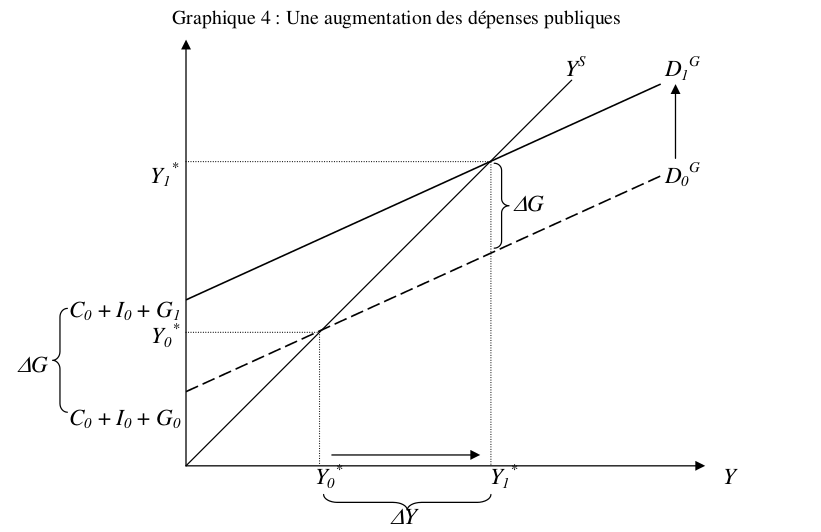
\includegraphics[width=12cm]{graph15.png}
\end{center}
Comment une augmentation des dépenses publiques peut-elle se traduire par une augmentation de plus d'un euro du revenu? La réponse est dans les composantes de la demande et en particulier dans la consommation : on a supposé que la consommation était une fonction croissante du revenu, par conséquent lorsque le gouvernement augmente la demande et le revenu d'un euro, il relance aussi la consommation qui augmente de $1 \times c$ euro. La demande augmente encore, ce qui augmente le revenu, ce qui augmente la consommation, etc. Le multiplicateur keynésien repose donc sur un \textit{cercle vertueux} :
\begin{center}
  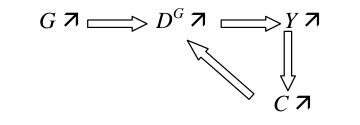
\includegraphics[width=6cm]{graph16.png}
\end{center}
A chaque tour du cercle, la demande augmente d'un montant supplémentaire inférieur à l'augmentation précédente du revenu parce qu'une partie de ce revenu supplémentaire est épargnée. elle sort donc du marché des biens, c'est pourquoi l'épargne est parfois considérée comme une fuite. Cette fuite est d'autant plus importante que la propension marginale à épargner est élevée. C'est pourquoi le multiplicateur est une fonction décroissante de la propension marginale à épargner. \\
Le résultat du multiplicateur a été obtenu en se concentrant sur les dépenses publiques mais il est applicable à n'importe quelle autre composante de la demande. On constate en effet que l'investissement et la demande incompressible occupent des places symétriques à celle des dépenses publiques dans l'expression du revenu d'équilibre. Par conséquent leur effet sur le revenu sera le même que celui des dépenses publiques. C'est pourquoi on parle autant de \textit{multiplicateur de dépenses} que du multiplicateur budgétaire. \\
Ces deux multiplicateurs diffèrent toutefois à partir du moment ou on tient compte du financement des dépenses publiques. Jusqu'à présent on a supposé que le gouvernement augmentait ses dépenses sans se soucier de les financer. La relance se faisait donc uniquement grâce à un creusement du déficit public. L'état ne peut cependant pas aggraver indéfiniment le déficit s'il veut respecter sa contrainte budgétaire. \\
On peut se demander si le multiplicateur keynésien fonctionnerait dans le cas ou le gouvernement maintiendrait son budget équilibré. Il faudrait pour cela qu'il augmente les impôts en même temps que ses dépenses. Il reprendrait alors d'une main ce qu'il donnerait de l'autre, ce qui affecterait énormément les effets d'une relance budgétaire. Pour le vérifier, supposons que le budget est équilibré en permanence et donc que les impôts couvrent exactement les dépenses : $G = T$. \\
Pour que les impôts soient correctement intégrés dans notre raisonnement, il faut tenir compte de leur effet sur le revenu disponible ($Y^D = Y - T$). La consommation sera alors donnée par :
$$ C = c.(Y - T) + C_0 $$
A cette différence près, on détermine le revenu d'équilibre comme précédemment : 
\begin{align*}
  Y^S & = D^G \\
  Y & = c.(Y-T) + c_0 + I_0 + G \\
  Y -c.Y & = -cT + C_0 + I_0 + G \\
  Y^* & = \frac{C_0 + I_0 + G - cT}{1-c}
\end{align*}
Or on sait à présent que $G = T$. On peut donc réécrire l'expression du revenu d'équilibre de la façon suivante :
$$ Y^* = \frac{C_0 + I_0 + G - cG}{1-c} = \frac{C_0 + I_0}{1 - c} + \frac{(1-c)G}{1-C} $$
\begin{center}
  $\Rightarrow$ \fbox{$Y^* = \frac{C_0 + I_0}{1 - c} + G$} 
\end{center}
On constate alors que le multiplicateur budgétaire est égal à $1$. C'est le \textit{théorème d'Haavelmo} : le multiplicateur budgétaire est égal à 1 lorsque le budget de l'état est équilibré.

\chapter{Le marché de la monnaie et les marchés financiers}
\section{Introduction : Ce qu'est la monnaie et ce qu'elle n'est pas}
\textit{Monnaie :} Tout actif qui est généralement accepté en paiement de biens et services ou en remboursement de dettes. \\
Cette définition est très large. Elle inclut bien évidement le cash, c'est à dire la \textit{monnaie fiduciaire}. Elle inclut aussi les \textit{dépôts à vue}, puisqu'on peut les utiliser directement pour régler ses achats, et la \textit{monnaie métallique} (en métaux précieux) et la \textit{monnaie marchandise} (plaques de sel, coquillages, bétail, ...). Par contre, cette définition souligne que la monnaie n'est synonyme ni de revenu, ni de patrimoine ou de richesse. \\
Le revenu est le flux qu'un individu peut consacrer à ses dépenses et à son épargne. Le patrimoine et la richesse représentent l'ensemble des actifs possédés par un individu (immobilier, titres, ...). Seule une partie du patrimoine est conservée sous forme de monnaie.
\section{L'offre de monnaie}
\subsection{Fonctions et formes de la monnaie}
\subsubsection{Les trois fonctions de la monnaie}
\begin{itemize}
  \item \textbf{La fonction d'intermédiaire des échanges :} \\
    Dans les économies actuelles, on utilise la monnaie à chacun de ses achats et le troc ne joue qu'un rôle exceptionnel. Ceci n'est possible que parce que le vendeur sait qu'il pourra échanger par la suite la monnaie qu'il a acquise contre des biens qui l'intéressent. La monnaie ne sert donc que d'\textit{intermédiaire des échanges} puisqu'elle n'est pas échangée pour elle même.
  \item \textbf{La fonction d'unité de compte :} \\
    La deuxième fonction de la monnaie est celle d'\textit{unité de compte}. Cette fonction implique que la monnaie soit utilisée pour mesurer la valeur de tous les biens et services de l'économie. Cela permet d'utiliser tous les prix en fonctions d'un bien (la monnaie) qu'on appelle le \textit{numéraire}.
  \item \textbf{La fonction de réserve de valeur :} \\
La troisième fonction économique de la monnaie est celle de \textit{réserve de valeur}. Cela signifie que la monnaie permet d'épargner du pouvoir d'achat entre le moment où un revenu est perçu et celui où il est dépensé. La monnaie est certainement une meilleure réserve de valeur que beaucoup d'autres biens qui se dégradent rapidement mais ne remplit ce rôle que de façon imparfaite puisqu'elle perd rapidement de la valeur en période d'inflation. D'autres biens remplissent cette fonction de manière bien plus satisfaisante (e.g. l'immobilier, les métaux précieux, les actions, \ldots).
\end{itemize}
Plus généralement, on peut trouver des biens susceptibles d'assurer chacune des fonctions de la monnaie, tout aussi bien sinon mieux. Il suffit pour cela qu'un bien présente certaines qualités (par exemple être divisible, transportable, standardisé et assez résistant). La monnaie telle qu'on la connaît présente ces qualités mais elle n'est pas la seule.
\subsubsection{L'évolution des formes de la monnaie}
Au fil des siècles les formes de la monnaie ont évolué et ont suivi un processus de \textit{dématérialisation}. Au départ, ce qui servait de monnaie était des marchandises qui avaient une valeur intrinsèque. Ces monnaies ont été remplacées par les monnaies métalliques qui avaient encore une valeur intrinsèque puisque les métaux ont d'autres utilisations. Elles étaient cependant plus pratiques à manipuler. Elles furent complétées par le papier-monnaie. \\
Une grande innovation fut l'invention de la \textit{monnaie fiduciaire}. Dans la mesure où le papier-monnaie est très rarement converti, il suffit qu'il soit accepté en payement pour avoir de la valeur. Il n'est pas nécessaire que le billet corresponde à une certaine quantité de métal précieux tant que ses utilisateurs ont confiance en sa capacité d'être accepté en règlement d'une dette. L'invention de la monnaie fiduciaire marque l'apparition de la monnaie moderne. \\
Une bonne manière pour l'état d'assurer de la valeur à une monnaie est de l'accepter en payement des impôts. \\
Parallèlement à la monnaie fiduciaire est apparue la \textit{monnaie scripturale}. Cette forme de monnaie repose sur de simples jeux d'écriture entre créditeurs et débiteurs. \\
De nos jours, la monnaie fiduciaire a remplacé la monnaie métallique dans toutes les économies du monde.
\subsubsection{La mesure de l'offre de monnaie}
Mesurer concrètement l'offre de monnaie est une tâche difficile parce que beaucoup d'actifs correspondent plus ou moins bien à sa définition et à ses trois fonctions. Ce qui distingue un compte épargne d'un compte courant est sa \textit{liquidité}, c'est à dire sa capacité à être converti rapidement en moyen d'échange. C'est pourquoi on ne définit pas un mais plusieurs \textit{agrégats monétaires} qui reposent sur une définition de plus en plus large de la monnaie. Ces agrégats fonctionnent comme des poupées russes qui englobent des actifs de moins en moins liquides : 
\begin{itemize}
  \item M1 : Monnaie fiduciaire et dépôts à vue.
  \item M2 : M1 \\
    + dépôts à terme d'une durée inférieure ou égale à 2 ans \\
    + dépôts remboursables avec préavis inférieur ou égal à 3 mois.
  \item M3 : M2 \\
    + pensions \\
    + titres d'OPCVM monétaires \\
    + titres de créance émis pour une durée inférieure ou égale à 2 ans.
\end{itemize}
Comme des innovations financières et des évolutions imprévues se produisent régulièrement, la définition des agrégats monétaires est révisée pour en tenir compte.
\subsection{La création monétaire}
\subsubsection{La création monétaire en l'absence de banques commerciales}
Supposons qu'il n'existe qu'une seule banque, la banque centrale. Cette banque détient le monopole d'émission de la monnaie fiduciaire. Pour mettre la monnaie en circulation elle ne peut se contenter de distribuer des billets au coin des rues. elle a besoin d'une \textit{contrepartie}. Cette contrepartie prend la forme de titres financiers (obligations, bons du trésor, actions, ...) que les agents vont lui vendre. Elle les paiera alors en leur donnant des billets qu'elle aura imprimés pour l'occasion. \\
Cette forme de mise sur le marché de monnaie s'appelle une opération d'\textit{open market}, parce que la BC intervient directement sur les marchés financiers pour acquérir des titres et distribuer de la monnaie. Les opérations d'open market permettent aussi de réduire la quantité de monnaie en circulation : il suffit que la BC vende des titres plutôt que d'en acheter. Elle récupère ainsi de la monnaie qu'elle a donc retiré de la circulation. \\
On peut retrouver la trace de ces opérations dans le bilan de la BC. Pour une banque, l'actif présente l'ensemble des créances qu'elle détient et le passif l'ensemble des dettes qu'elle a contractées. \\
Supposons à présent que la BC ait mis en circulation un millier d'euros de billets. Cela suppose qu'elle ait acheté pour un millier d'euros de titres. Il apparaît donc un millier d'euros de titres à son actif. Pour acquérir ces titres, elle a du créer un millier d'euros de billets qui vont donc apparaître à son passif. On peut aussi faire remarquer que les billets sont une forme de dette de la BC qui pourra à l'avenir être amenée à les échanger contre des titres. \\
Le bilan de la banque centrale se présente donc la façon suivante : 
\begin{center} 
  \begin{tabular}{c|c}
    Actif & Passif \\
    \hline
    Titres : 1000 & Billets : 1000
  \end{tabular}
\end{center}
La quantité de monnaie en circulation correspond donc exactement à la quantité de titres rachetée par la banque centrale.
\subsubsection{La création monétaire en présence de banques commerciales}
On l'a vu, la monnaie ne se résume pas aux billets. La majeure partie de la monnaie en circulation aujourd'hui prend la forme de soldes sur des comptes bancaires.  \\
Pour intégrer le rôle des banques et des dépôts, il faut comprendre comment les banquiers gagnent leur vie. Leur ressource principale vient des intérêts perçus sur les prêts accordés à leurs clients. La question est alors de savoir d'où proviennent les fonds que les banquiers utilisent pour leurs prêts. Il viennent des dépôts. \\
En effet, une banque sait que tous les fonds qui ont été déposés sur ses comptes ne vont pratiquement jamais être retirés en même temps. Elle peut donc en prêter une partie sans cesser de faire face aux demandes de retrait. Elle percevra donc des intérêts sur les fonds prêtes. Les banquiers ont donc intérêt à prêter une partie aussi importante que possible de leurs dépôts. \\
Cependant, si une banque prêtait toute la monnaie qui lui a été confiée elle ne pourrait plus faire face aux retraits et se retrouverait en faillite. C'est pourquoi une banque conserve toujours une partie de ses dépôts sous forme de monnaie. C'est ce qu'on appelle ses \textit{réserves} ou sa \textit{trésorerie}. \\
La législation complète souvent la prudence des banques en imposant un montant minimum de réserves, sous la forme d'un \textit{coefficient de réserves obligatoires} ou \textit{coefficient de trésorerie}. Ce coefficient donne aux banques la valeur minimum du ratio entre leurs réserves et leurs dépôts. Ainsi, la loi oblige les banques à respecter l'inégalité suivante :
$$\frac{reserves}{depots} \geq coefficient~de~reserves~obligatoires$$
Imaginons une économie dans laquelle la monnaie peut prendre la forme de billets et de dépôts à vue, et où le coefficient de réserves obligatoires a été fixé à $10\%$. Supposons par ailleurs qu'il existe 3 banques (A, B et C) dans cette économie et que les individus qui composent cette économie ne détiennent jamais de liquide et n'utilisent donc que la monnaie scripturale pour leurs payements. \\
Imaginons à présent que la BC vient d'imprimer 1000 euros qu'elle a utilisés pour acheter des obligations à une entreprise (opération d'open market) et voyons quel va être l'effet de cette création de monnaie sur la masse monétaire. \\
L'entreprise va utiliser ces 1000 euros pour payer l'un de ses fournisseurs qui va alors les déposer auprès de la banque A. Le bilan de cette dernière est alors affect de la façon suivante : 
\begin{center}
  Banque A \\
  \begin{tabular}{c|c}
    Actif & Passif \\
    \hline
    Réserves : 1000 & Dépôts : 1000
  \end{tabular}
\end{center}
La banque A ne ferait aucun profit si elle en restait là. Elle va donc prêter une partie de ses réserves affin de percevoir un intérêt. Si elle souhaite maximiser les intérêts perçus elle prêtera tout ce que la loi lui autorise, c'est à dire qu'elle respectera tout juste le coefficient de réserves obligatoires.
\begin{center}
  Banque A \\
  \begin{tabular}{c|c}
    Actif & Passif \\
    \hline
    Réserves : 100 & Dépôts : 1000 \\
    Crédits : 900 & 
  \end{tabular}
\end{center}
Elle a donc pu prêter 900\euro~ à l'un de ses clients qui va les dépenser auprès d'une entreprise qui est cliente de la banque B. Cette entreprise déposera les 900\euro~auprès de sa banque dont le bilan sera :
\begin{center}
  Banque B \\
  \begin{tabular}{c|c}
    Actif & Passif \\
    \hline
    Réserves : 900 & Dépôts : 900
  \end{tabular}
\end{center}
Comme elle ne souhaite pas non plus laisser dormir des fonds elle va prêter $90\%$ des 900\euro~:
\begin{center}
  Banque B \\
  \begin{tabular}{c|c}
    Actif & Passif \\
    \hline
    Réserves : 90 & Dépôts : 810 \\
    Crédits : 810 & 
  \end{tabular}
\end{center}
Les 810\euro~vont se retrouver dans les coffres de la banquer C lorsqu'ils auront été dépenses : 
\begin{center}
  Banque C \\
  \begin{tabular}{c|c}
    Actif & Passif \\
    \hline
    Réserves : 810 & Dépôts : 810
  \end{tabular}
\end{center}
Et comme la banque C va aussi prêter ses billets son bilan va devenir :
\begin{center}
  Banque C \\
  \begin{tabular}{c|c}
    Actif & Passif \\
    \hline
    Réserves : 81 & Dépôts : 810 \\
    Crédits : 729 & 
  \end{tabular}
\end{center}
L'une des deux autres banques retrouvera les 729\euro~sous forme de dépôts mais en prêtera $90\%$, etc. \\
Puisque la masse monétaire est composée des billets et des dépôts, on peut donc dire que l'augmentation totale du volume des dépôts sera de :
\begin{align*}
  \Delta M & = 1000 + 0,9 \times 1000 + 0,9^2 \times 1000 + 0,9^3 \times 1000 + 0,9^4 \times 1000 + ... + 0,9^n \times 1000 \\
  \Delta M & = 1000 + 900 + 810 + 729 + 656,1 + ...
\end{align*}
On montre facilement que cette somme tend vers 10 000 lorsque $n \rightarrow \infty$. L'augmentation du montant des dépôts est donc dix fois supérieure à celle du montant des billets. Comme les dépôts sont une partie de la masse monétaire, on peut voir que les banques commerciales créent de la monnaie. \\
On aurait pu prévoir le rapport de 1 à 10 entre la quantité de billets imprimés et l'augmentation de la quantité des dépôts car ce rapport correspond précisément à l'inverse du coefficient de réserves obligatoires. Dans cette économie simplifiée l'augmentation des dépôts est donc égale à la quantité de billets créée divisée par le coefficient de réserves obligatoires. Plus généralement, on peut dire que le volume des dépôts ($D$) est égal à celui des réserves ($R$) divisé par le coefficient de réserves obligatoires ($\Theta$) puisque tous les billets en circulation ont été créés à un moment où un autre :
$$ D = \frac{R}{\Theta}$$
Cette expression est trop irréaliste car elle repose sur l'hypothèse très forte que les agents ne conservent jamais de billets. De plus, elle limite l'activité de la BC à l'impression de monnaie. Pourtant, les BC accordent également des crédits et ces crédits peuvent aussi servir de réserves. On appelle d'ailleurs \textit{monnaie banque centrale} ou \textit{base monétaire} la somme des billets et des crédits accordés par la banque centrale. \\
Supposons qu'une fraction $c_b$ de la masse monétaire est détenue sous forme de billets, le complément étant conservé sous forme de dépôts. Si $M$ représente la masse monétaire et $E$ la quantité émise de billets on peut écrire : 
\begin{align*}
  E & = c_b.M \\
  D & = (1 - c_b)M
\end{align*}
Par ailleurs, la monnaie banque centrale peut être utilisée soit par les ménages sous forme de billets, soit par les banques commerciales sous forme de réserves. Si on note $H$ la monnaie banque centrale on peut alors écrire
$$ H = E + R$$
Or on sait que les réserves sont proportionnelles aux dépôts. On peut donc réécrire l'expression de $H$ :
$$ H = E + \Theta D $$
On peut ensuite remplacer $E$ et $D$ par leur valeur et exprimer la masse monétaire en fonction de la base monétaire : 
\begin{align*}
  H & = c_b.M + \Theta (1 - c_b)M \\
  H & = (c_b + \Theta (1 - c_b))M 
\end{align*}
%\begin{Large}
  \begin{center}
    $\Rightarrow$ \fbox{$M = \frac{1}{c_b + \Theta (1 - c_b)} H$} 
  \end{center}
%\end{Large}
Comme $c_b$ et $\Theta$ sont des paramètres, cette expression montre que la masse monétaire est proportionnelle à la base monétaire. De plus, le dénominateur est inférieur à 1. Par conséquent, le coefficient de proportionnalité est sans ambiguïté supérieur à 1. C'est pourquoi on l'appelle le \textit{multiplicateur monétaire}. Il signifie qu'une augmentation donnée de la base monétaire se traduit par une augmentation supérieure de la masse monétaire.
\subsection{Les moyens de contrôle de l'offre de monnaie}
On vient de constater que ce sont les banques commerciales qui créent la majeure partie de la monnaie en circulation mais ça ne signifie pas pour autant que ce sont elles qui contrôlent la majeure partie de la monnaie en circulation. En effet, la BC dispose d'une batterie d'instruments qui lui permettent de contrôler la quantité de monnaie en circulation. 
\begin{enumerate}
  \item \textbf{Les opérations d'open market} \\
    Le principe des opérations d'open market est d'échanger de la monnaie banque centrale aux banques commerciales contre des titres. Les banques s'y livrent lorsqu'elles ont besoin de liquidités. Ces opérations s'apparentent à un prêt à la différence qu'elles supposent que les emprunteurs déposent une garantie. Il ne s'agit pas d'un prêt en blanc. Comme tout prêt, ces opérations donnent lieu au versement d'un intérêt. \\
    Pour encourager les banques à avoir recours à ces prêts la BC peut ajuster son taux d'intérêt. Plus ce taux sera bas, plus les banques commerciales seront tentées à demander des liquidités à la BC qui pourra alors écouler une quantité plus importante de la monnaie. On voit donc que la BC dispose d'un instrument supplémentaire de contrôle de la base monétaire : le taux d'intérêt sur les opérations de refinancement des banques commerciales. \\
    Dans la zone euro, ce taux d'intérêt est le \textit{taux directeur} principal et on l'appelle le \textit{Refi}.
  \item \textbf{Les réserves obligatoires} \\
    Si on reprends la formule du multiplicateur monétaire et qu'on suppose que la base monétaire est donnée, la masse monétaire devient une fonction décroissante de $\Theta$. Par conséquent, la BC peut ajuster la masse monétaire en circulation en manipulant le coefficient de réserves obligatoires. Si elle réduit ce coefficient, les banques pourront accorder plus de crédits avec les mêmes réserves. Si, au contraire, le coefficient augmente les banques seront contraintes d'accorder moins de prêts. Les dépôts augmentent dans le premier cas et diminuent dans le second. \\
  \item \textbf{Les facilités permanentes} \\
    Les \textit{facilités permanentes} sont des possibilités supplémentaires de gérer leurs liquidités offertes aux banques commerciales par la banque centrale. Il s'agit schématiquement de prêts et de dépôts. A la différence des opérations d'open market, les facilités permanentes ne passent pas par le marché mais par des relations bilatérales entre une banque commerciale et la BC. Ici ce sont les banques commerciales qui ont l'initiative. \\
    En général, ces opérations sont conçues pour n'être utilisées que de façon exceptionnelle et à très court terme (une journée) par les banques commerciales. Les prêts sont donc très chers et les dépôts très mal rémunérés. C'est pourquoi les taux d'intérêt qui leur sont appliqués sont les taux directeurs plafond et plancher de la banque centrale. Ils déterminent l'intervalle dans lequel le taux d'intérêt du marché va fluctuer. Les facilités permanentes permettent un réglage encore plus fin de la politique monétaire que les opérations d'open market. \\
    Dans la zone euro, les facilités permanentes sont appelées \textit{facilités marginales}. Le taux d'intérêt pratiqué sur les facilités marginales de prêts est le taux directeur plafond de la zone et celui pratiqué sur les facilités marginales de dépôt en constituent le taux d'intérêt plancher. Voilà pourquoi il y a trois taux directeurs dans la zone euro au lieu d'un seul.
\end{enumerate}
Les BC disposent donc d'une batterie d'instruments qui leur permettent d'influencer la quantité de monnaie en circulation même si elles n'en créent qu'une faible partie.

\section{La demande de monnaie}
Ce qu'on appelle demande de monnaie correspond à la quantité de liquidité que souhaitent détenir les agents. elle dépend donc de la répartition des avoirs entre différents actifs. Parfois un agent va souhaiter détenir un actif non rémunéré (la monnaie) plutôt que des actifs rémunérés car elle rend des services. \\
N'importe quel actif peut être détenu à la place de la monnaie, mais on ne va considérer ici que les \textit{obligations} comme actif alternatif à la monnaie. Les obligations sont des \textit{titres de créance négociables} qui assurent le versement d'un intérêt à échéance. Ce sont donc des actifs qui proposent une rémunération sans risque et qui peuvent être achetés et revendus. Ces caractéristiques seront importantes au moment de déterminer l'impact du taux d'intérêt sur la demande de monnaie. Le taux d'intérêt dont nous parlerons sera donc le taux d'intérêt sur les obligations.
\subsection{La théorie quantitative de la monnaie}
La \textit{théorie quantitative de la monnaie} (TQM) a été développée par les économistes classiques et néoclassiques mais on en trouve déjà l'intuition chez les mercantilistes.
\subsubsection{La quantité de monnaie nécessaire aux transactions}
Dans une économie monétaire il est nécessaire de détenir de la monnaie pour réaliser la moindre transaction. Cependant, puisque la monnaie ne rapporte rien alors que les titres proposent une rémunération positive, les agents ne détiendront que le strict minimum de ce qui est nécessaire aux transactions. Pour certains, toute encaisse monétaire détenue en plus de ce qui est indispensable pour les transaction serait irrationnelle puisqu'elle impliquerait la perte inutile d'un intérêt. \\
Par conséquent, la demande de monnaie sera proportionnelle à la valeur des transactions exprimées en unités monétaires. Si on note $T$ le nombre de transactions et $P$ le niveau général des prix (qui mesure le prix moyen des transactions), la quantité de monnaie demandée pourra s'écrire :
$$M^d = \phi . P . T$$
$\phi$ est un paramètre positif dont la signification apparaît en manipulant cette expression :
$$\phi = \frac{M^d}{PT}$$
On voit donc que $\phi$ mesure le nombre moyen d'unités monétaires nécessaires pour réaliser une transaction d'une valeur d'une unité monétaire. Par exemple, si au cours d'une année on a utilisé 10.000.000.000\euro~en billets pour les transactions mais que la valeur des transactions s'est établie à 20.000.000.000\euro~, $\phi$ sera égal à $\frac{1}{2}$. Cela signifie qu'il aura suffit de 0.50\euro~pour réaliser 1\euro~de transaction. \\
Par conséquent, chaque euro aura été utilisé deux fois au cours de la période. Le nombre moyen d'utilisations de chaque unité monétaire est appelé la \textit{vitesse de circulation de la monnaie} :$ V \equiv \frac{1}{\phi}$
On peut alors réécrire la demande de monnaie :
$$M^d = \frac{P.T}{V}$$
C'est \textit{l'équation des échanges}. Elle est difficile à utiliser empiriquement car on ne connaît pas le nombre de transactions. Par contre, il est raisonnable de considérer que le nombre de transactions est proportionnel au volume de la production. C'est pourquoi on remplace le nombre de transactions par la production :
$$M^d = \frac{P.Y}{V}$$
Il apparaît alors que la demande de monnaie est une fonction croissante de la production et des prix, et décroissante de la vitesse de circulation de la monnaie. Sous cette forme, l'équation des échanges est appelée \textit{équation de Cambridge}.
\subsubsection{La relation entre la masse monétaire et les prix}
La demande de monnaie telle que définie précédemment est tautologique, mais en rajoutant  quelques hypothèses complémentaires elle peut fournir une théorie de l'évolution des prix. Elle permet en effet d'établir la TQM. \\
On peut considérer que la vitesse de circulation est un paramètre stable. En effet, il est déterminé par des facteurs structurels tels que les habitudes de paiement ou le niveau de développement du système bancaire. Ça ne signifie pas forcément que la vitesse de circulation de la monnaie est constante, mais qu'elle ne dépend pas de l'évolution des autres variables qui apparaissent dans l'équation de Cambridge. \\
Si on considère de plus que l'économie utilise toutes ses capacités de production et qu'il n'y a pas de sous emploi, le revenu sera lui aussi un paramètre de l'équation.\\
Dans ce cas, les deux variables qui pourront s'ajuster pour assurer l'égalité des deux membres de l'équation de Cambridge sont la masse monétaire et les prix. Comme la masse monétaire est contrôlée par la BC ce sont les prix qui s'ajusteront pour maintenir l'égalité. On peut donc exprimer les prix en fonction de la masse monétaire :
$$ P = \frac{MV}{Y} $$
La TQM implique donc que les prix sont proportionnels à la masse monétaire. Plus précisément, il existe un lien de causalité entre la masse monétaire et le niveaux des prix. Toute augmentation de la masse monétaire provoque une augmentation des prix, et ne provoque que ça. La TQM implique donc une séparation entre les variables nominales et réelles. On appelle \textit{dichotomie entre la sphère nominale et la sphère réelle} cette séparation. \\
On a par ailleurs pris l'habitude d'exprimer la TQM en utilisant non le niveau des variables mais leur taux de variation. Le taux d'inflation devient alors une fonction du taux de croissance de la masse monétaire. Si on utilise une lettre minuscule pour désigner les taux de variation d'une variable, la TQM s'écrit :
$$ p = m + v - y$$
On a vu précédemment que l'économie pouvait se trouver en situation de sous emploi à court terme  cause de la rigidité des prix. On verra que la politique monétaire peut alors influencer le niveau de production. La TQM n'est en principe pertinente que pour réfléchir çà la relation de long terme entre le niveau des prix et la masse monétaire puisqu'elle repose sur l'hypothèse de plein emploi. \\
Il existe des situations dans lesquelles la TQM est utilisable même à court terme. Ce sont les situations \textit{d'hyperinflation}. On parle d'hyperinflation lorsque le taux d'inflation atteint les $50\%$ par mois. Pendant ces périodes, il est extrêmement coûteux de fixer les prix. Par conséquent, tous les agents révisent leurs prix en permanence et les prix peuvent être considérés comme flexibles même à court terme. La TQM est donc applicable. \\
S'il peut exister des causes réelles à l'inflation, on peut affirmer que l'hyperinflation trouve toujours son origine dans la création excessive de monnaie.
\subsection{La préférence pour la liquidité}
\subsubsection{Le motif de transaction}
On peut considérer que les agents détiennent de la monnaie parce qu'ils doivent en utiliser pour leurs transactions. C'est le \textit{motif de transaction}. Ce motif de détention de la monnaie s'impose à la fois aux ménages et aux entreprises. Keynes parle du motif de revenu pour les premiers et du motif d'entreprise pour les secondes. Ces deux demandes de liquidité s'additionnent pour former la demande de monnaie à des fins de transaction. \\
Comme le nombre de transactions augmente avec le volume de production, la demande de monnaie à des fins de transaction sera une fonction croissante du revenu.
\subsubsection{Le motif de précaution}
Le \textit{motif de précaution} est défini par Keynes par : \og Le souci de parer aux éventualités qui exigent des dépenses inopinées, l'espoir de profiter d'occasions imprévues pour réaliser des achats avantageux et enfin le désir de conserver une richesse d'une valeur immuable pour faire face à une obligation future stipulée en monnaie sont autant de nouveaux motifs à conserver de l'argent \fg .\\
On conserve donc de la monnaie parce qu'on ne peut prévoir toutes les transactions qu'on va être amené à effectuer. Détenir de la liquidité a donc une utilité puisque ça permet de profiter de bonnes affaires imprévues et de faire face à une obligation inopinée. \\
Ce motif de détention apparaît dès qu'on tient compte de l'incertitude dans laquelle se tient l'activité économique. \\
Le motif de précaution fait apparaître une nouvelle variable susceptible d'affecter la demande de monnaie : le \textit{taux d'intérêt nominal}. En effet, puisque la détention de monnaie a une utilité, les agents détiendraient toutes leurs encaisses sous forme liquide si ça n'avait pas un coût. Ce coût est le coût d'opportunité de la liquidité, soit le taux d'intérêt. A chaque fois qu'un agent décide de détenir un euro supplémentaire sous forme liquide, il renonce aux intérêts que lui aurait rapporté cet euro s'il avait été conservé sous forme de titres. \\
Les agents doivent donc arbitrer entre l'utilité de la liquidité et son coût d'opportunité. Par conséquent, plus le taux d'intérêt sera élevé moins les agents conserveront de monnaie. La demande de monnaie de précaution est donc une fonction décroissante du taux d'intérêt sur les titres. \\
\subsubsection{Le motif de spéculation}
La spéculation consiste à acheter un actif pour le revendre en espérant réaliser une plus-value. Un spéculateur chercher donc à acheter des titres au prix le plus faible pour les revendre au prix le plus élevé. La grande innovation qu'apporte Keynes a l'analyse de la demande de monnaie est de montrer que la spéculation sur le marché des titres implique un motif supplémentaire de détenir de la monnaie. Ce \textit{motif de spéculation} amène à préciser la relation entre la demande de monnaie et le taux d'intérêt. Pour cela, il faut comprendre qu'il existe une relation précise entre le prix des titres et le taux d'intérêt courant. \\
La particularité d'une obligation est d'être un titre de créance négociable. On achète donc le titre en sachant qu'on obtiendra en échange une somme donnée à l'échéance. On sait cependant qu'on peut très bien la revendre avant l'échéance. Dans ce cas, c'est l'acheteur de l'obligation qui bénéficiera du versement de la somme à l'échéance. \\
Considérons une obligation émise par l'entreprise A le $1^{er}$ janvier à 10h au taux d'intérêt en vigueur sur le marché à ce moment là, soit $10\%$. Chaque obligation est vendue initialement au prix de 100\euro. C'est la \textit{valeur faciale} de l'obligation. Sa date d'échéance est fixée au 31 décembre. L'entreprise A émet donc des titres qui garantissent à leur porteur le versement d'une somme de 100 + 10 = 110\euro~le 31 décembre. Une minute plus tard, le taux d'intérêt est passé à $20\%$. C'est le moment que choisit l'entreprise B pour émettre des obligations donc les caractéristiques sont les mêmes que celles de l'entreprise A. La différence est que l'entreprise B ne peut vendre ses obligations que si elle propose au moins le même rendement que le marché, soit $20\%$. Par conséquent, les acheteurs d'une obligation B obtiendront 120\euro~le 31 décembre. Les détenteurs d'obligations A ont alors intérêt à les revendre pour acheter des obligations B qui offrent un meilleur rendement. Le prix des obligations A va donc baisser, mais cette baisse ne se poursuit pas indéfiniment. au fur et à mesure que le prix des obligations A baisse, leur rendement augmente. A l'équilibre, il faut que le rendement des obligations A et B soit le même. C'est la condition d'\textit{arbitrage}. \\
Chaque euro consacré à l'achat d'obligation B rapporte $\frac{100+20}{100} = 1,2$\euro~le 31 décembre. Si le prix de revente de l'obligation A est $P_A$, chaque euro consacré à l'achat d'obligation A va rapporter $\frac{100+10}{P_A}$. L'arbitrage assure que les deux rendements soient égaux : $\frac{110}{P_A} = 1,2 \Rightarrow \frac{110}{1,2} \cong 91,66$\euro. \\
On constate donc que l'augmentation du taux d'intérêt s'est traduite par une diminution du prix de l'obligation A. On peut généraliser cette relation. Soit $VF_A$ la valeur faciale d'une obligation et $i_A$ le taux d'intérêt au moment de son émission. Soit $i$ le taux d'intérêt courant sur les obligations émises par la suite mais de même échéance. Si $P_A$ est le prix de revente de l'obligation A, son rendement va être égal à :
$$ rdt = \frac{VF(A+i_A) - P_A}{P_A}$$
Puisque le rendement l'obligation A doit en permanence être égal à celui des obligations émises par la suite, on peut écrire $rdt=i$ et résoudre l'équation pour obtenir l'expression du prix auquel l'obligation se négocie :
$$ P_A = \frac{i+i_A}{1+i}VF$$
On retrouve une relation négative entre le taux d'intérêt courant et le prix de l'obligation A. Cette relation va nous permettre de déterminer l'influence du taux d'intérêt sur la demande de monnaie à des fins de spéculation et donc la forme de la fonction de demande de monnaie à des fins de spéculation. \\
Si le taux d'intérêt est élevé, le prix des titres serra bas. Une forte proportion des spéculateurs anticipera donc une augmentation du prix des titres et cherchera à acheter des titres, c'est à dire à se débarrasser de leur monnaie. La demande de monnaie sera donc faible. \\
Si le taux d'intérêt est bas, le prix des titres sera élevé. Une forte proportion des spéculateurs anticipera donc une baisse du prix des titres et cherchera à en vendre, c'est à dire à les échanger contre de la monnaie. La demande de monnaie sera donc forte. \\
On voit donc qu'il existe une deuxième raison pour laquelle la relation entre demande de monnaie et taux d'intérêt est décroissante. Cette raison dépend du comportement des spéculateurs. \\
L'impact du taux d'intérêt sur la demande de monnaie à des fins de spéculations est plus complexe que ça. En effet, le prix des titres ne peut augmenter indéfiniment. Par conséquent, une fois que le taux d'intérêt sera devenu suffisamment faible, le prix des titres sera tellement élevé que tous les spéculateurs anticiperont un retournement de tendance au même moment. ainsi, ils chercher tous à vendre leurs titras. La demande de monnaie sera alors très importante et infiniment élastique au taux d'intérêt. \\
Cette situation est qualifié de \textit{trappe à liquidités} parce que les spéculateurs absorbent toute la liquidité qui est mise sur le marché. Le taux d'intérêt atteint donc une valeur minimum. \\
On voit donc que la relation entre la demande de monnaie à des fins de spéculation et le taux d'intérêt est fortement non linéaire, ce qui se répercutera sur la demande totale de monnaie.
\subsubsection{La fonction de demande de liquidité}
La demande totale de liquidité est la somme de la demande de monnaie à des fins de transactions, de la demande à des fins de précaution et de la demande à des fins de spéculation. La première est proportionnelle au revenu nominal et les deux autres diminuent lorsque le taux d'intérêt augmente. \\
Une façon simple de tenir compte de tous les déterminants de la demande de monnaie est la suivante :
$$M^d = L(i)PY$$
où $L$ est la somme de la demande de monnaie de précaution et de la demande de monnaie de spéculation. C'est une fonction décroissante de $i$, le taux d'intérêt nominal.  \\
Traditionnellement on exprime la demande de monnaie en termes réels. On parle alors de \textit{demande d'encaisses réelles}. Cette demande d'encaisses réelles représente intuitivement le ``pouvoir d'achat'' de la quantité de monnaie détenue, c'est à dire la quantité de biens que les encaisses monétaire permettraient d'acquérir instantanément. \\
On obtient facilement la fonction de demande d'encaisses réelles en visant les deux membres de l'expression précédente par le niveau des prix $P$ :
$$M^D \equiv \frac{M^d}{P} = L(i)Y$$
La demande d'encaisses réelles est donc une fonction du taux d'intérêt et du revenu national exprimé en termes réels. Compte tenu de nos hypothèses on peut représenter graphiquement la demande d'encaisses réelles :
\begin{center}
  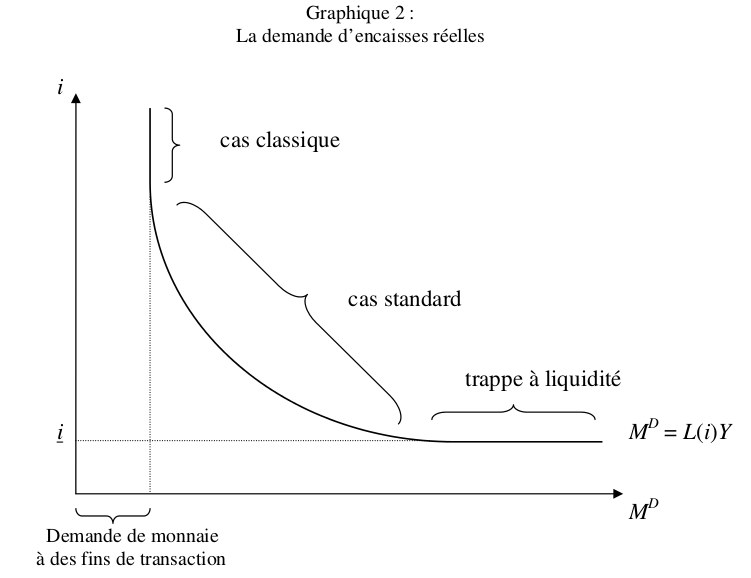
\includegraphics[width=12cm]{graph17.png}
\end{center}
On voit que la demande passe par trois phases. Lorsque le taux d'intérêt est très faible, on a une situation de trappe à liquidité. La demande de monnaie est alors infiniment élastique au taux d'intérêt et ce dernier atteint une valeur plancher $\underline{i}$. \\
Lorsque le taux d'intérêt est très élevé, la demande de monnaie à des fins de spéculation et la demande de monnaie de précaution sont presque nulles. La demande de monnaie se résume alors à la demande de monnaie à des fins de transaction, qui ne dépend que du revenu. L'élasticité de la demande de monnaie au taux d'intérêt est alors nulle. \\
Entre ces deux situations, la demande de monnaie est une fonction décroissante du taux d'intérêt. on peut parler du cas standard. \\
NB: Traditionnellement, on note $i$ le taux d'intérêt nominal et $r$ le taux d'intérêt réel. Le taux d'intérêt nominal mesure le nombre d'unités monétaires reçues en intérêt pour un prêt initial d'un euro. Le taux d'intérêt réel corrige l'impact de l'inflation et mesure donc la quantité de biens reçue en intérêts pour l'équivalent d'une unité de biens prêtée. \\
comme le coût d'opportunité de la détention de monnaie est le taux d'intérêt nominal, c'est ce taux que les agents prennent en compte dans leurs décisions de détenir plus ou moins d'encaisses. C'est pourquoi on utilisera ici le taux d'intérêt nominal. Beaucoup notent $r$ le taux d'intérêt lorsqu'ils présentent le marché de la monnaie et le modèle IS-LM. Tant que les prix sont fixes, comme c'est le cas ici, cette différence n'a aucune importance puisque le taux d'intérêt nominal et le taux d'intérêt réel sont alors égaux.
\section{La détermination du taux d'intérêt}
\subsection{L'équilibre sur le marché de la monnaie}
L'équilibre sur le marché de la monnaie est atteint lorsque l'offre de monnaie est égale à la demande. Comme c'est le taux d'intérêt qui est déterminé sur ce marché, c'est lui qui va s'ajuster pour réaliser l'équilibre. Pour décrire comment on atteint l'équilibre, on va donc représenter l'offre et la demande de monnaie en fonction du taux d'intérêt. \\
On a décrit la relation entre le taux d'intérêt et la demande d'encaisses réelles précédemment. On a aussi vu que l'offre de monnaie est contrôlée par la BC. L'offre d'encaisses réelles, qui est égale à la masse monétaire divisée par le niveau des prix ($\frac{M}{P}$), est donc exogène au marché de la monnaie. Elle est par conséquent représentée par une droite verticale dans le repère ($M,i$) dans lequel on a déjà tracé la demande de monnaie.
\begin{center}
  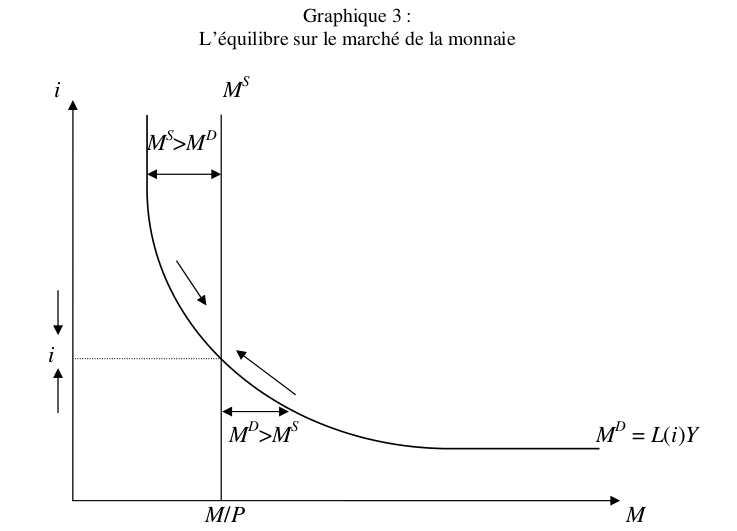
\includegraphics[width=12cm]{graph18.png}
\end{center}
Compte tenu de nos hypothèses, il n'existe qu'une seule valeur du taux d'intérêt pour laquelle la demande d'encaisses réelles est égale à l'offre d'encaisses réelles. En effet, le taux d'intérêt d'équilibre est déterminé par une seule intersection entre la courbe de demande de monnaie et la droite qui représente l'offre de monnaie. \\
On peut de plus constater que l'équilibre est stable. Si le taux d'intérêt est supérieur au taux d'intérêt d'équilibre, l'offre d'encaisses réelles est supérieure à la demande. Le taux d'intérêt diminue donc pour que la demande puisse absorber cette offre excédentaire. \\
Si le taux d'intérêt est inférieur au taux d'intérêt d'équilibre, la demande d'encaisses réelles est supérieure à l'offre et le taux d'intérêt va alors augmenter pour réduire la demande. \\
Par conséquent, le taux d'intérêt retourne toujours vers son niveau d'équilibre en cas de déséquilibre.
\subsection{L'impact d'une augmentation de l'offre de monnaie}
On peut maintenant réfléchir à la façon dont des perturbations exogènes au marché de la monnaie vont affecter la détermination du taux d'intérêt. Commençons par réfléchir à l'impact d'une augmentation de l'offre de monnaie. Une telle augmentation est décidée par la BC, il s'agit donc d'une décision de politique monétaire.
\begin{center}
  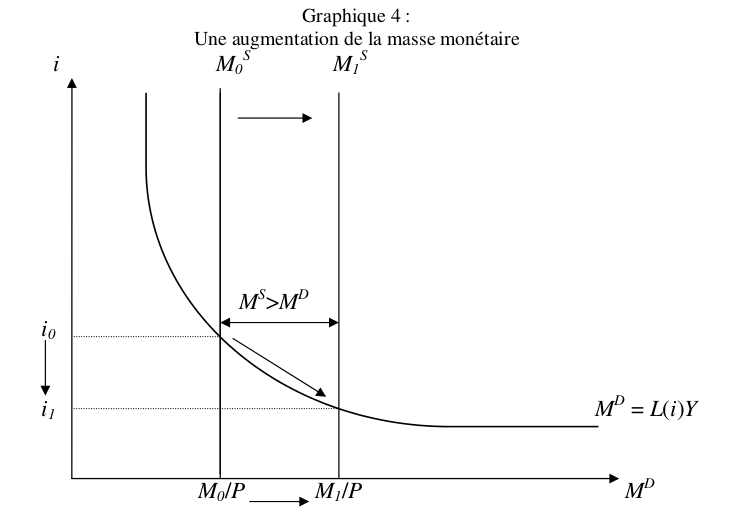
\includegraphics[width=12cm]{graph19.png}
\end{center}
L'augmentation de la masse monétaire se traduit par une augmentation de l'offre d'encaisses réelles. Elle passe de $\frac{M_0}{P}$ à $\frac{M_1}{P}$. Ceci va provoquer une offre excédentaire d'encaisses réelles et il va falloir que la demande de monnaie augmente pour la résorber. le taux d'intérêt va donc diminuer et on atteindra un nouvel équilibre, caractérisé par un taux d'intérêt plus faible que le taux d'intérêt initial ($i_1 < i_0$). \\
On peut donc conclure qu'une augmentation de l'offre de monnaie se traduit par une diminution du taux d'intérêt. Or on a vu que l'investissement est une fonction décroissante du taux d'intérêt, donc l'investissement va augmenter, ce qui va augmenter la demande globale et éventuellement relancer l'activité. C'est pourquoi une politique d'augmentation de l'offre de monnaie est qualifiée de \textit{politique monétaire expansionniste}.\\
On peut lire le graphique à l'envers et supposer que la BC réduit l'offre de monnaie. Dans ce cas, l'offre d'encaisses réelles passe de $\frac{M_1}{P}$ à $\frac{M_0}{P}$. Il s'ensuit que le taux d'intérêt augmente pour passer de $i_1$ à $i_0$, ce qui va restreindre l'investissement, la demande et l'activité. On parle donc le \textit{politique monétaire restrictive}. \\
Ce résultat n'est cependant pas valable lorsque l'économie est en situation de trappe à liquidités. Dans ce cas, la droite d'offre de monnaie coupe la courbe de demande de monnaie dans sa partie horizontale. L'augmentation de l'offre de monnaie est donc sans effet sur le taux d'intérêt qui ne peut pas passer en dessous de sa valeur minimum.
\subsection{L'impact d'une augmentation du revenu}
La politique monétaire n'est pas la seule source d'évolution sur le marché de la monnaie. Dans la mesure où la demande d'encaisses réelles est une fonction du revenu, toute augmentation de l'activité augmentera également la demande d'encaisses réelles.
\begin{center}
  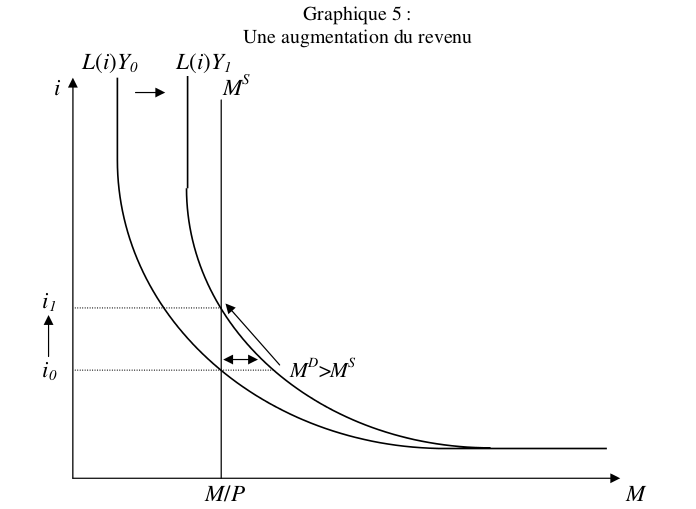
\includegraphics[width=12cm]{graph20.png}
\end{center}
Ici, l'augmentation du revenu se traduit par un déplacement de la courbe de demande de monnaie vers le nord-est. Ce déplacement signifie que la demande de monnaie est supérieure à son niveau initial quel que soit le taux d'intérêt considéré. Cependant, la partie horizontale de la demande de monnaie qui correspond à la situation de trappe à liquidité n'est pas affectée. \\
L'augmentation du revenu se traduit alors instantanément par une demande excédentaire d'encaisses réelles et le taux d'intérêt va augmenter pour la résorber. LA demande de monnaie de précaution à des fins de précaution et de spéculation diminue et on retrouve l'équilibre. \\
On constate donc qu'une augmentation du revenu se traduit par une augmentation du taux d'intérêt ($i_1 > i_0$). A l'inverse, si on lisait le graphique à l'envers on observerait qu'une diminution du revenu se traduirait par une diminution du taux d'intérêt. \\
Ici encore, ce résultat n'est pas valable lorsque l'économie se trouve en situation de trappe à liquidité. Dans ce cas, la droite d'offre de monnaie coupe la courbe de demande de monnaie dans sa partie horizontale. L'augmentation de la demande de monnaie est donc alors sans effet sur le taux d'intérêt.


\chapter{Le modèle IS-LM}
\section{Introduction}
Ce modèle a été proposé par Hicks pour formaliser l'analyse de l'interdépendance des marchés des biens et de la monnaie. Il a été développé par la suite par Hansen, c'est pourquoi on parle parfois du diagramme de Hicks et Hansen. \\
Ce modèle fournit encore la logique de base des modèles macroéconomiques qui sont utilisés à des fins de prévisions. Il décrit aussi les principaux mécanismes à l'oeuvre lorsqu'une politique de gestion de la demande globale est appliquée et se prête à un grand nombre d'extensions, ce qui étend son pouvoir explicatif. Il conserve enfin des qualités pédagogiques certaines car il permet de traiter très simplement des phénomènes relativement complexes. \\
Le modèle IS-LM est constitué de deux blocs principaux : la courbe IS qui décrit l'équilibre sur le marché des biens, et la courbe LM qui décrit l'équilibre sur le marché de la monnaie.
\section{Construction du diagramme IS-LM}
\subsection{La courbe IS}
Elle représente l'équilibre sur le marché des biens. On va l'obtenir à partir de l'égalité entre la demande et la production de biens, mais on pourrait aussi partir de l'égalité entre l'épargne et l'investissement (IS signifie Investment et Savings).
\subsubsection{Pourquoi IS est décroissante}
La courbe IS regroupe \textit{toutes les combinaisons du revenu et du taux d'intérêt qui assurent l'équilibre sur le marché des biens}. Plus précisément, elle représente l'ensemble des valeurs d'équilibre du revenu pour chaque valeur possible du taux d'intérêt. En d'autres termes, elle décrit le revenu déterminé de façon endogène sur le marché des biens pour chaque valeur du taux d'intérêt qui est exogène à ce marché. \\
Précédemment, on a supposé que l'investissement était exogène sur le marché des biens. Cette hypothèse n'est plus tenable si on étudie l'équilibre de toute l'économie au lieu de se concentrer sur le marché des biens. Si on rappelle que l'investissement dépends du taux d'intérêt on obtient l'équation de la courbe IS :
$$ Y = C(Y) + I(i) + G$$
Cette équation permet de définir IS de façon algébrique mais l'intuition de ce que représente cette courbe peut être saisie graphiquement. Pour construire la courbe IS, il faut repartir de l'équilibre sur le marché des biens, c'est à dire du diagramme à 45 degrés et y représenter l'impact d'une variation du taux d'intérêt. La courbe IS se représente cependant dans un autre repère que le diagramme à 45 degrés. \\
Le graphique ci dessous est donc constitué de deux repères superposés. Celui du dessus permet de tracer le diagramme à 45 degrés et celui du dessous est consacré à la courbe IS. Ce repère mesure le revenu en abscisses et le taux d'intérêt en ordonnées. \\
Supposons que le taux d'intérêt augmente d'un montant arbitraire pour passer de $i_0$ à $i_1$ ($i_1 > i_0$). Cette variation exogène du taux d'intérêt va inciter les entreprises à réduire leurs investissements, ce qui réduit la demande globale et déplace ainsi la courbe de demande globale vers le bas. On constate alors que le revenu d'équilibre a diminué ($Y_1 < Y_0$).
\begin{center}
  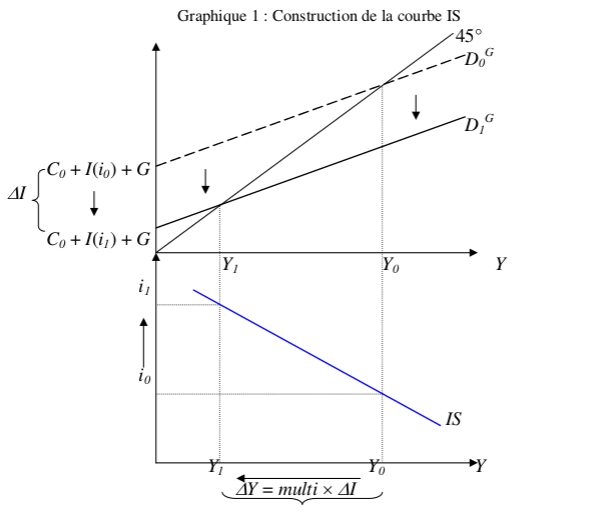
\includegraphics[width=12cm]{graph21.png}
\end{center}
Si on reporte les valeurs du taux d'intérêt et du revenu d'équilibre dans le repère du dessous, et qu'on les relie on constate que \textbf{la courbe IS est décroissante}. La logique de construction de la courbe IS est résumée par l'enchaînement ci dessous :
\begin{center}
  
\includegraphics[width=12cm]{graph22.png}
\end{center}
L'augmentation du taux d'intérêt réduit l'investissement, ce qui déprime la demande globale. La production s'ajuste à la demande, ce qui réduit le revenu puis la consommation. Il s'enclenche alors un mécanisme multiplicateur qui amplifie la réduction initiale de l'investissement. On peut donc conclure que la diminution de la production va être égale à la variation de l'investissement multipliée par le multiplicateur des dépenses ($\Delta Y = multi \times \Delta I$).
\subsubsection{Forme et position de la courbe IS}
Même si nous la représentons par une droite, la courbe IS est bien une courbe qui peut prendre n'importe quelle forme. La seule de ses caractéristiques dont nous pouvons être surs est qu'elle est décroissante. On la représente par une droite parce que c'est plus simple et parce qu'on suppose que la consommation est une fonction linéaire du revenu. \\
Il faut garder à l'esprit qu'il ne s'agit là que d'une simplification dont les vertus sont essentiellement pédagogiques même si nos conclusions seraient les mêmes si on utilisait des courbes IS de forme différente.
\paragraph{Forme de la courbe IS}
La pente de la courbe IS représente la sensibilité du revenu d'équilibre sur le marché des biens aux variations du taux d'intérêt. Il s'agit donc d'un paramètre essentiel qui mesure la puissance du canal de transmission entre le marché de la monnaie et celui des biens. \\
Pour isoler les paramètres qui déterminent la pente de la courbe IS, il suffit de reprendre l'enchaînement des effets qui transforment une variation du taux d'intérêt en une variation du revenu :
\begin{center}
  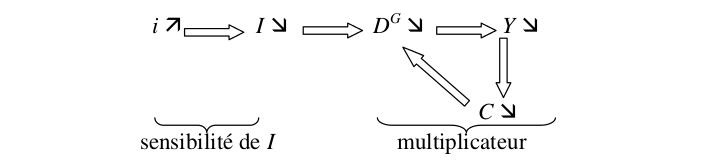
\includegraphics[width=12cm]{graph23.png}
\end{center}
Le graphique suggère qu'on peut diviser l'effet total du taux d'intérêt en deux effets élémentaires : un effet direct du taux d'intérêt sur l'investissement et un effet induit qui dépend de la valeur du multiplicateur. \\
Par conséquent, l'effet total sera d'autant plus fort que l'effet multiplicateur sera puissant. Comme on a vu que l'effet multiplicateur dépend de la propension marginale à consommer, on peut affirmer que l'effet total sera d'autant plus fort que la propension marginale à consommer sera élevée. \\
Si ces deux effets sont plus puissants, un même augmentation du taux d'intérêt aura un effet plus important et la courbe IS sera donc plus plate. \\
Pour s'en convaincre, considérons deux économies (A et B) qui connaissent au départ le même revenu et le même taux d'intérêt ($Y_0, i_0$) et supposons que le taux d'intérêt augmente de la même façon dans les deux économies ($i_1 > i_0$). Supposons que la propension marginale à consommer soit plus élevée et que l'investissement soit plus sensible au taux d'intérêt dans la seconde économie que dans la première. Ça signifie que l'augmentation du taux d'intérêt déprimera plus le revenu dans l'économie B que dans l'économie A :
\begin{center}
  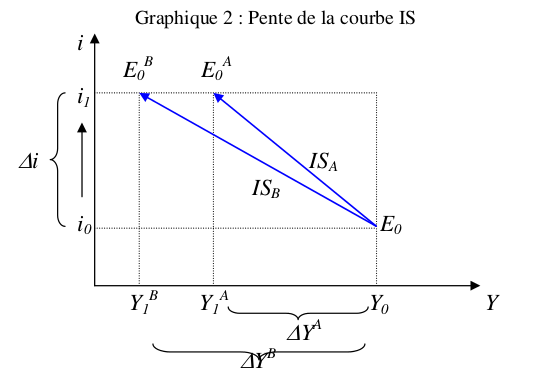
\includegraphics[width=12cm]{graph24.png}
\end{center}
Il apparaît donc que puisque le revenu de l'économie B est plus affecté que celui de l'économie A par la même augmentation du taux d'intérêt, la courbe IS de l'économie sera moins raide que celle de l'économie A. \\
En résumé, on peut dire qu'une sensibilité plus importante de l'investissement aux variations du taux d'intérêt et/ou une propension marginale à consommer plus élevée se traduiront par une courbe IS moins raide. Cette conclusion est importante parce qu'elle indique deux paramètres qu'il serait utile d'estimer empiriquement pour prévoir l'impact d'une diminution des taux d'intérêt.
\paragraph{Position de la courbe IS}
La position de la courbe IS dans le repère ($Y,i$) se modifie dès que l'un des paramètres qui déterminent la position de la courbe de demande globale se modifie. Dans le cas linéaire sur lequel nous nous concentrons, les déplacements de la courbe $D^G$ peuvent être dus à une modification de la consommation incompressible ($C_0$) ou des dépenses publiques ($G$). Toute évolution du comportement des investisseurs qui les amènerait à modifier le volume de leurs investisseurs indépendamment de la valeur du taux d'intérêt aurait le même effet. \\
Plus concrètement, supposons que les dépenses publiques augmentent ($G_1 > G_0$) alors que le taux d'intérêt reste constant ($i_0$). La demande globale augmente alors et la courbe de demande globale se déplace vers le haut. On constate alors que le revenu d'équilibre a augmenté ($Y_1 > Y_0$) grâce à l'effet multiplicateur.
\begin{center}
  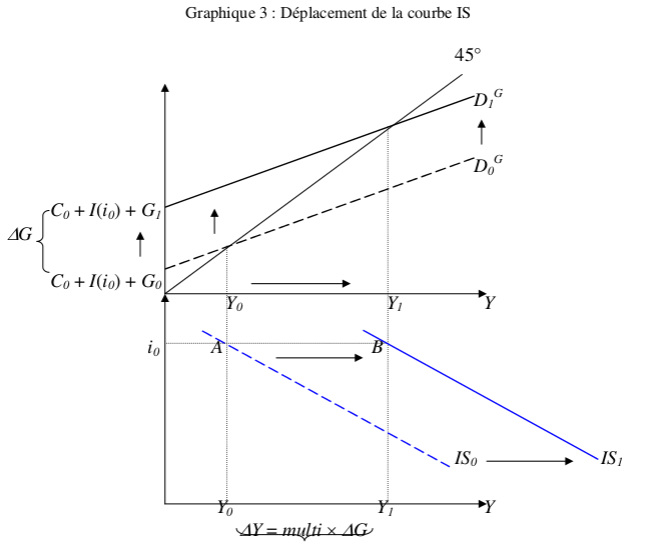
\includegraphics[width=12cm]{graph25.png}
\end{center}
Lorsqu'on reporte cette augmentation dans le repère inférieur on passe du point A au point B. Comme le choix du taux d'intérêt initial était arbitraire, on pourrait recommencer le même exercice pour n'importe quelle valeur du taux d'intérêt. Dans tous les cas l'augmentation du revenu serait rigoureusement la même puisqu'elle est égale à l'augmentation des dépenses multipliée par le multiplicateur. La nouvelle courbe IS est pas conséquent parallèle à l'ancienne. \textbf{Une augmentation des dépenses publiques se traduit donc par une translation de la courbe IS vers la droite}. \\
On peut aussi lire le graphique à l'envers pour décrire les effets d'une réduction des dépenses publiques. \textbf{Une diminution des dépenses publiques se traduit donc par une translation de la courbe IS vers la gauche}.
\subsection{La courbe LM}
La courbe LM représente l'équilibre sur le marché de la monnaie. On va l'obtenir à partir de l'égalité entre la demande de liquidité et l'offre de monnaie. Les initiales LM signifient justement ``Liquidity'' et ``money''. \\
\subsubsection{Pourquoi LM est croissante}
La courbe LM regroupe \textit{toutes les combinaisons du revenu et du taux d'intérêt qui assurent l'équilibre sur le marché de la monnaie}. Plus précisément, elle représente l'ensemble des valeurs d'équilibre du taux d'intérêt pour chaque valeur possible du revenu. En d'autres termes elle décrit le taux d'intérêt déterminé de façon endogène sur le marché de la monnaie pour chaque valeur du revenu qui est exogène à ce marché. \\
La courbe LM est tracée dans le même repère ($Y,i$) que la courbe IS. Il s'agit donc de reporter le taux d'intérêt déterminé sur le marché de la monnaie pour chacune des valeurs possibles du revenu. La construction de la courbe LM part donc de l'équilibre sur ce marché de la monnaie. Algébriquement, on pourrait l'étudier grâce à la condition d'équilibre de ce marché :
$$ \frac{M}{P} = L(i)Y$$
Cette équation permet de définir LM de façon algébrique, mais l'intuition de ce que représente cette courbe peut être saisie graphiquement. Le graphique suivant est composé de deux repères disposés l'un à coté de l'autre. Celui de gauche permet de représenter l'équilibre sur le marché de la monnaie. Celui de droite est consacré à la courbe LM. Ce repère mesure le revenu en abscisses et le taux d'intérêt en ordonnées.
\begin{center}
  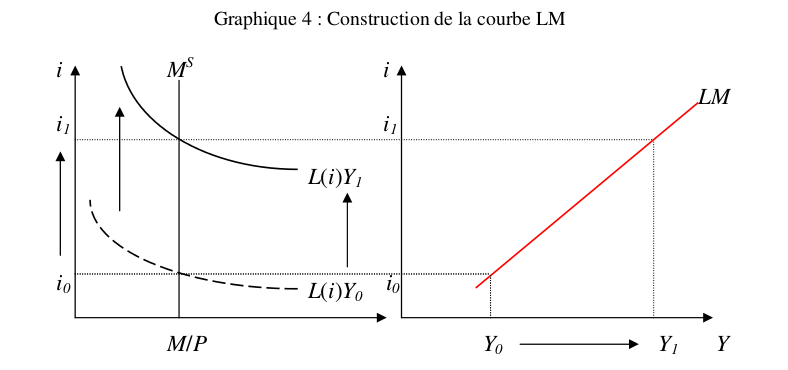
\includegraphics[width=12cm]{graph26.png}
\end{center}
Supposons que le revenu augmente d'un montant arbitraire pour passer de $Y_0$ à $Y_1$ ($Y_1 > Y_0$). Cette variation exogène du revenu va augmenter la demande de monnaie à des fins de transactions, ce qui déplace la courbe de demande vers le haut. On constate alors que le taux d'intérêt d'équilibre a augmenté ($i_1 > i_0$). \\
Si on reporte les valeurs du taux d'intérêt et du revenu d'équilibre dans le repère de droite et qu'on les relie on constate que \textbf{la courbe LM est croissante}. \\
La logique de construction de la courbe LM est résumée par l'enchaînement suivant :
\begin{center}
  
\includegraphics[width=12cm]{graph27.png}
\end{center}
L'augmentation du revenu augmente les besoins de monnaie pour les transactions. Il apparaît alors une demande excédentaire de liquidité qui provoque à son tour une augmentation du taux d'intérêt. Comme le taux d'intérêt augmente, la demande de monnaie de précaution et spéculative diminue. On retourne ainsi à l'équilibre sur le marché de la monnaie.
\subsubsection{Forme et position de la courbe LM}
\paragraph{Forme de la courbe LM}
La pente de la courbe LM représente la sensibilité du taux d'intérêt d'équilibre sur le marché de la monnaie aux variations du revenu. Il s'agit donc d'un paramètre essentiel qui mesure la puissance du canal de transmission entre le marché des biens et celui de la monnaie. \\
Pour isoler les paramètres qui déterminent la pente de la courbe LM, il suffit de reprendre l'enchaînement des effets qui transforment une variation du revenu en une variation du taux d'intérêt.
\begin{center}
  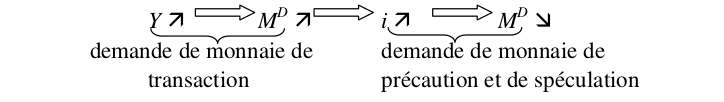
\includegraphics[width=12cm]{graph28.png}
\end{center}
L'enchaînement suggère qu'on peut diviser l'effet total du revenu en deux effets élémentaires : un effet du revenu sur la demande de monnaie à des fins de transaction et un effet indirect sur la demande de monnaie de précaution et à des fins de spéculation. \\
Plus la demande de monnaie à des fins de transaction sera sensible aux variations du revenu, plus l'augmentation de la demande de monnaie sera forte. Il faudra alors une forte augmentation du taux d'intérêt pour rétablir l'équilibre sur le marché de la monnaie, en réduisant la demande de monnaie aux fins de précaution et spéculation. \\
De même, si la demande de monnaie de précaution et à des fins de spéculation est peu sensible aux variations du taux d'intérêt il faudra aussi une forte augmentation du taux d'intérêt pour réduire la demande. \\
Par conséquent, on peut dire que plus la demande de monnaie sera sensible aux variations du revenu et peu sensible aux variations du taux d'intérêt plus une même augmentation du revenu provoquera une augmentation importante du taux d'intérêt. La courbe LM sera donc d'autant plus raide que la demande de monnaie sera sensible aux variations du revenu et peu sensible aux variations du nouveau taux d'intérêt. \\
Pour s'en persuader, considérons à nouveau deux économies (A et B) qui connaissent au départ le même revenu et le même taux d'intérêt ($Y_0,i_0$), et supposons que le revenu augmente de la même façon dans les deux économies ($Y_1 > Y_0$). Supposons que la demande de monnaie soit plus sensible aux variations du revenu et moins sensible aux variations du taux d'intérêt dans l'économie B que dans l'économie A.
\begin{center}
  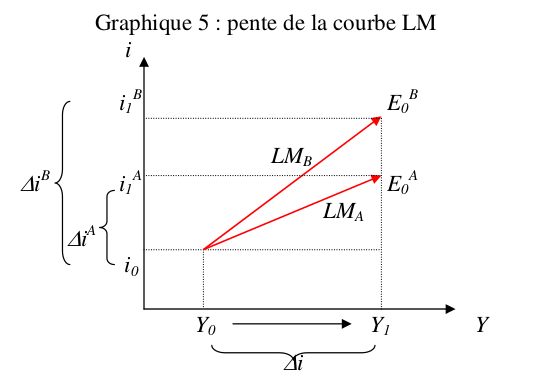
\includegraphics[width=12cm]{graph29.png}
\end{center}
Il apparaît donc que puisque le taux d'intérêt de l'économie B est plus affecté que celui de l'économie A par la même augmentation du revenu, la courbe LM de l'économie B sera plus raide que celle de l'économie A. \\
On souligné précédemment que la relation entre la demande de monnaie et le taux d'intérêt est non linéaire. Plus précisément, la demande devient infiniment sensible au taux d'intérêt lorsque le taux est très faible à cause de la trappe à liquidités. Elle y devient insensible lorsque le tauxd'intéret est très élevé car il ne subsiste plus que la demande de monnaie de transaction. D'après la relation que nous venons d'analyser entre la pente de la courbe LM et la sensibilité au taux d'intérêt de la demande de monnaie, cela implique que la pente de la courbe LM ne sera pas constante.
\begin{center}
  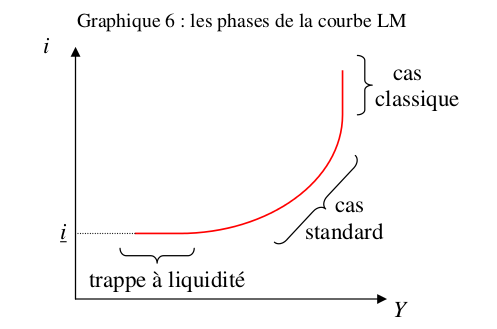
\includegraphics[width=12cm]{graph30.png}
\end{center}
Au contraire, la pente de la courbe LM sera très faible pour de faibles valeurs du taux d'intérêt et très élevée pour des valeurs élevées du taux d'intérêt. Comme la demande de monnaie, la courbe LM passera par plusieurs phases. \\
Pour de faibles valeurs du taux d'intérêt et du revenu, la courbe LM est horizontale. C'est la situation de la trappe à liquidités. Pour des valeurs plus élevées du taux d'intérêt et du revenu, LM est verticale : c'est le cas classique. Et entre les deux extrêmes, la courbe LM est croissante. \\
\paragraph{Position de la courbe LM}
Le principal paramètre qui détermine la position de la courbe LM dans le repère ($Y,i$) est l'offre de monnaie. \\
Supposons ainsi que la banque centrale augmente la masse monétaire ($M_1 > M_0$) alors que le revenu $Y_0$ reste constant. La droite d'offre d'encaisses réelles se déplace alors vers la droite. On constate alors l'apparition d'une offre excédentaire d'encaisses réelles. Le marché de la monnaie ne retrouvera son équilibre que si le taux d'intérêt diminue afin d'inciter les agents à augmenter leurs encaisses ($i_1 < i_0$).
\begin{center}
  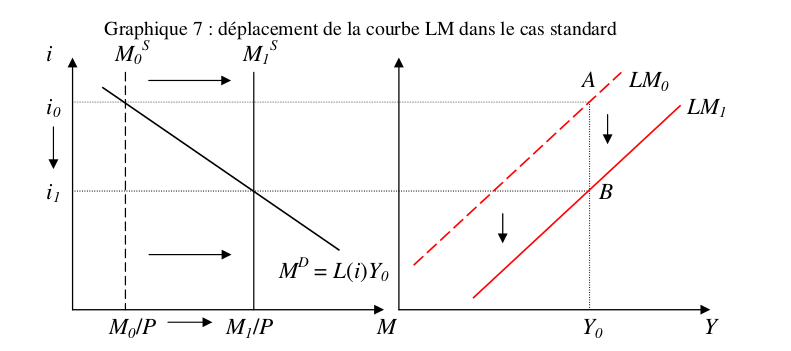
\includegraphics[width=12cm]{graph31.png}
\end{center}
Lorsqu'on reporte cette augmentation dans le repère de droite, on passe du point A au point B. Comme le choix du revenu initial était arbitraire, on pourrait recommencer le même exercice pour n'importe quelle valeur du revenu. La nouvelle courbe LM est par conséquent parallèle à l'ancienne. \textbf{Une augmentation de la masse monétaire se traduit donc par une translation de la courbe LM vers le bas}. \\
On peut aussi lire le graphique à l'envers pour décrire les effets d'une contraction de la masse monétaire. \textbf{Une contraction de la masse monétaire se traduit par une translation de la courbe LM vers le haut}. \\
Ces résultats ne sont cependant pas vrais tout au long de la courbe LM. En effet, si le taux d'intérêt initial est trop faible, l'économie se trouvera en situation de trappe à liquidité. L'offre supplémentaire de monnaie sera donc absorbée par les spéculateurs sans pour autant diminuer le taux d'intérêt. On peut donc dire qu'une augmentation de l'offre de monnaie n'affectera pas la partie horizontale de la courbe LM.
\subsection{L'équilibre global}
Pour respecter la contrainte de bouclage, il est nécessaire de déterminer l'équilibre conjoint des deux marchés. C'est ce qu'on appelle \textit{l'équilibre global} de l'économie. \\
Cet équilibre global s'obtient en représentant les courbes IS et LM dans le même graphique, ce qui est possible puisqu'elles sont tracées dans le même repère. Comme l'équilibre global de l'économie suppose que les deux marchés soient en équilibre, il sera représenté par un point qui appartient aux deux courbes à la fois. L'équilibre global correspond donc à l'intersection entre la courbe IS et la courbe LM.
\begin{center}
  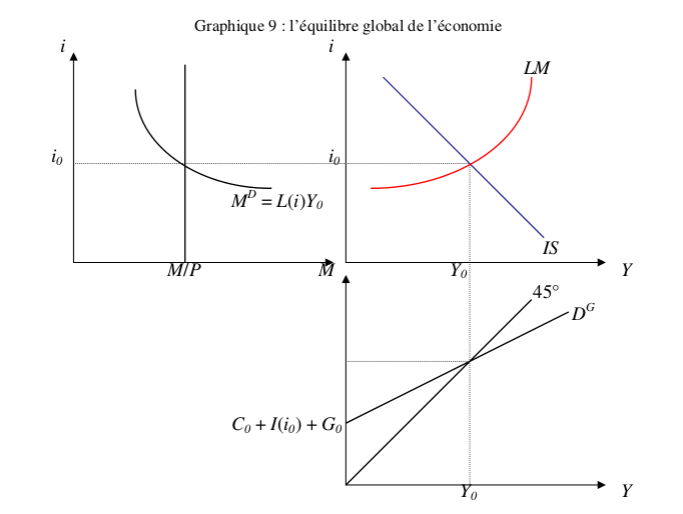
\includegraphics[width=12cm]{graph32.png}
\end{center}
Ce graphique montre qu'au point d'intersection entre les courbes IS et LM le marché de la monnaie et celui des biens sont conjointement en équilibre. On a donc déterminé à la fois le revenu et le taux d'intérêt d'équilibre ($Y_0,i_0$). comme l'équilibre sur ces deux marchés est stable, l'équilibre global sera stable lui aussi. Il ne se modifiera que si l'un ou l'autre des paramètres du modèle est modifié. \\
L'intérêt du modèle IS-LM est qu'il synthétise l'équilibre de deux marchés en un seul diagramme. \\
Rien ne permet d'affirmer que le revenu d'équilibre correspond au plein emploi.

\section{La politique économique dans le modèle IS-LM}
Le diagramme IS-LM permet de traiter facilement deux types de politiques de demande : La politique monétaire et la politique budgétaire. Ces deux politiques peuvent se compléter ou se contrecarrer, il peut donc être intéressant d'analyser aussi le \textit{policy-mix} dans son ensemble.
\subsection{La politique monétaire}
La politique monétaire consiste à manipuler l'offre de monnaie dans l'espoir d'affecter le revenu. Elle peut tout aussi bien consister dans une expansion de la masse monétaire (politique monétaire expansionniste) que dans une contraction de la masse monétaire (politique monétaire restrictive). On va s'intéresser ici aux effets d'une politique monétaire expansionniste, les effets d'une politique monétaire restrictive pouvant d'obtenir par symétrie.
\subsubsection{Principe de la politique monétaire}
Une politique monétaire expansionniste consiste à augmenter l'offre de monnaie dans l'espoir de faire baisser les taux d'intérêt et de relancer l'activité.
\begin{center}
  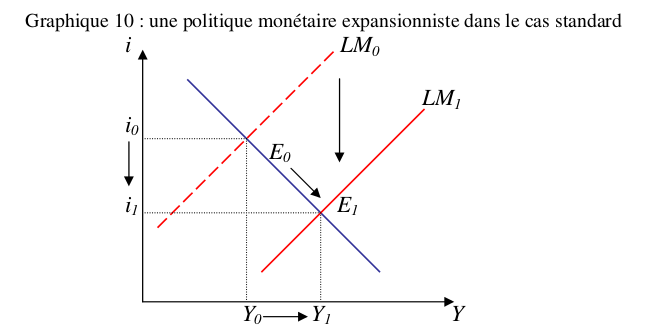
\includegraphics[width=12cm]{graph33.png}
\end{center}
Considérons le cas standard, dans lequel la courbe LM est croissante et la courbe IS décroissante. Dans ce cas, l'augmentation de la masse monétaire provoque une offre excédentaire d'encaisses réelles qui ne se résorbe qu'à condition que le taux d'intérêt diminue. On a vu que cela se traduisait par une translation vers le bas de la courbe LM. Le diagramme IS-LM permet d'en visualiser toutes les conséquence. \\
Le graphique montre que \textbf{une politique monétaire expansionniste provoque à la fois une diminution du taux d'intérêt ($i_1 < i_0$) et une augmentation du revenu ($Y_1 > Y_0$)}. \\
Ce résultat est fondamental et le diagramme IS-LM ne permet pas à lui seul d'en comprendre les mécanismes. \\
L'augmentation de la masse monétaire crée une offre excédentaire de monnaie qui provoque une diminution du taux d'intérêt. L'effet de la politique est alors transmis au marché des biens par l'investissement. La demande globale augmente, ce qui incite les entreprises à produire d'avantage. Le revenu augmente, ce qui relance la consommation et enclenche un effet multiplicateur.
\begin{center}
  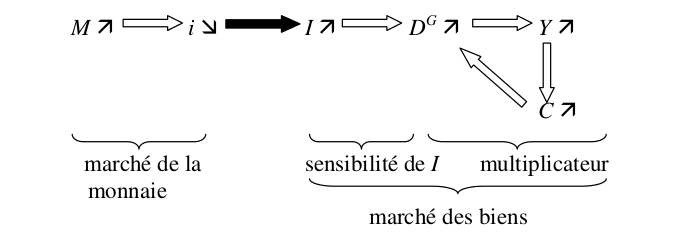
\includegraphics[width=12cm]{graph34.png}
\end{center}
C'est donc le taux d'intérêt qui constitue le canal de transmission entre la sphère monétaire et la sphère réelle.
\subsubsection{Efficacité de la politique monétaire}
L'efficacité de la politique monétaire se mesure par l'augmentation du revenu que permet l'augmentation de la masse monétaire. La politique monétaire aura un effet plus ou moins important sur le revenu en fonction de des facteurs qui affectent le canal de transmission entre les deux marchés. Il s'agit là des facteurs qui déterminent la pente de la courbe IS, mais le fonctionnement du marché de la monnaie joue aussi un role. \\
Pour visualiser ce résultat, comparons deux pays qui partent de la même situation, avec la même courbe LM, et qaui mettent en oeuvre la même politique monétaire expansionniste. Supposons que la courbe IS du pays B est moins raide que celle du pays A. Nous savons que cela peut etre du soit au fait que l'investissement est plus sensible aux taux d'intérêt et/ou que la propension marginale à consommer est plus élevée dans le pays B que dans le pays A.
\begin{center}
  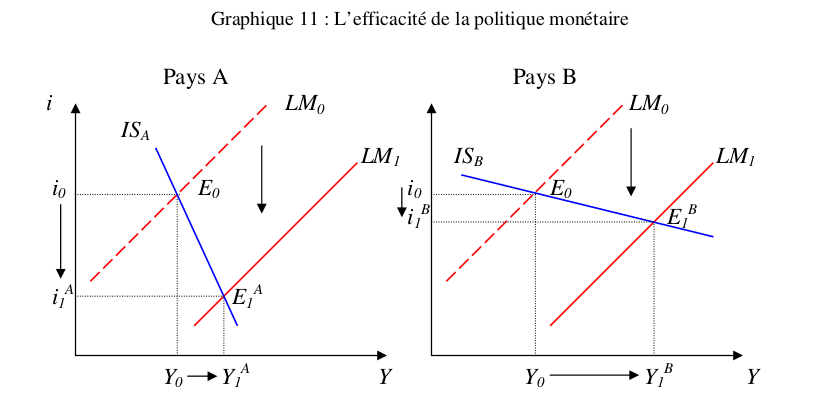
\includegraphics[width=12cm]{graph35.png}
\end{center}
Ce graphique permet deux constats. D'abord, plus la courbe IS est raide moins la politique monétaire est efficace. L'augmentation du revenu est en effet plus faible dans le pays A que dans le pays B. Ce résultat était prévisible puisque la pente de la courbe IS de ce pays indique que l'investissement y est très sensible au taux d'intérêt et/ou que le multiplicateur y est puissant. \\
On peut donc conclure que \textbf{la politique monétaire est d'autant plus efficace que l'investissement est sensible au taux d'intéret et la propension marginale à consommer est élevée}. \\
On constateaussi que le taux d'intéret a moins diminué dans le pays B que dans le pays A. Ca s'explique si on réalise que le raisonnement qui nous a permis de prévoir l'effet d'une augmentation de l'offre de monnaie sur le revenu est incomplet. En effet, il ne tient pas compte de l'impact de l'augmentation du revenu sur la demande de monnaie de transaction. \\
Si on tient compte de ce dernier effet, on réalise que la demande de monnaie doit augmenter, ce qui compense un peu l'augmentation de la masse monétaire. Le taux d'intérêt va donc être plus élevé que ce que nous aurions prévu en nous concentrant simplement sur le marché des biens. \\
Comme le revenu augmente plus dans le pays B que dans le pays A, l'augmentation de la demande de monnaie y sera forcément plus importante, ce qui fait que le taux d'intérêt y diminuera donc moins. \\
Ces conlusions sont valables dans le cas standard. Cependant, si on veut déterminer les conditions d'efficacité de la politique monétaire de façon exhaustive, on doit tenir compte d'une situation particulière que nous avons déjà évoqué : la trappe à liquidité. Le graphique suivant permet de visualiser l'effet d'une politique monétaire lorsque l'économie se trouve en situation de trappe à liquidité. Dans ce cas, la courbe IS coupe initialement la courbe LM dans sa portion horizontale : \begin{center}
  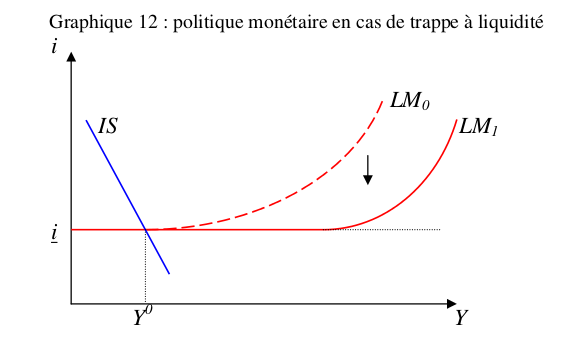
\includegraphics[width=12cm]{graph36.png}
\end{center}
L'augmentation de la masse monétaire déplace la portion croissante de la courbe LM vers le bas mais n'affecte pas sa portion horizontale. Par conséquent, l'équilibre de l'économie n'est pas modifié. On peut donc conclure que \textbf{la politique monétaire est inefficace en situation de trappe à liquidité}. \\
Intuitivement, lorsque l'économie est en situation de trappe à liquidité, les spéculateurs absorbent instantanément tout la liquidité que la BC peut créer. Par conséquent, le taux d'intérêt reste constant, ce qui empêche la politique monétaire d'affecter le marché des biens. Les effets de la politique monétaire restent donc alors circonscrits au seul marché de la monnaie.
\subsection{La politique budgétaire}
La politique budgétaire consiste à manipuler les dépenses publiques pour affecter la demande globale. Elle peut tout aussi bien consister dans une augmentation des dépenses (politique budgétaire expansionniste) qu'en leur réduction (politique budgétaire restrictive). Tout comme pour la politique monétaire, on ne couvre ici que les effets d'une politique budgétaire expansionniste puisque les effets d'une politique budgétaire restrictive peuvent s'obtenir par symétrie.
\subsubsection{Principe de la politique budgétaire}
Une politique budgétaire expansionniste consiste à augmenter les dépenses publiques dans l'espoir d'augmenter la demande et relancer l'activité. Considérons le cas standard, dans lequel la courbe LM est croissante et la courbe IS décroissante. Dans ce cas, l'augmentation des dépenses relance la demande gloable, ce qui provoque une translation de la courbe IS vers la droite, l'ampleur de se déplacement correspondant à l'effet multiplicateur :
\begin{center}
  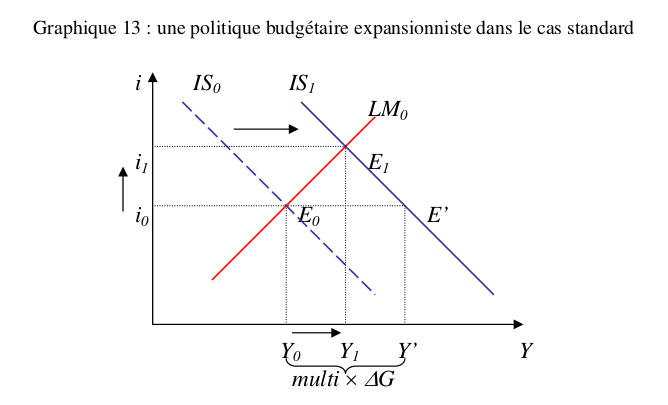
\includegraphics[width=12cm]{graph37.png}
\end{center}
Ce graphique montre qu'\textbf{une politique budgétaire expansionniste provoque une augmentation à la fois du revenu ($Y_1 > Y_0$) et du taux d'intérêt ($i_1 > i_0$)}. \\
On peut cependant aussi remarquer que \textbf{l'augmentation du revenu est inférieure à celle que l'effet multiplicateur aurait laissé prévoir ($Y_1 < Y'$)}. Ce résultat n'est pas fondamental mais le graphique ci dessus ne suffit pas pour comprendre en les mécanismes :
\begin{center}
  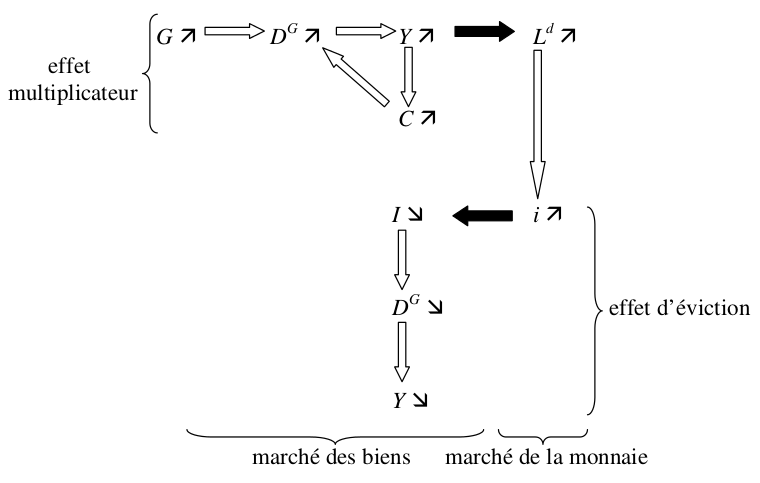
\includegraphics[width=12cm]{graph38.png}
\end{center}
L'augmentation des dépenses publiques augmente la demande globale. La production va donc augmenter pour satisfaire la demande supplémentaire. Comme la production augmente, le revenu augmente lui aussi, ce qui se répercute sur la consommation et enclenche un effet multiplicateur. La nouveauté ici est que l'augmentation du revenu va se répercuter sur le marché de la monnaie parce que la demande de monnaie de transaction augmente. Il apparaît alors une demande excédentaire de monnaie qui ne peut se résorber que grâce à une augmentation du taux d'intérêt. \\
Cette augmentation du taux d'intérêt va à son tour se répercuter sur le marché des biens en déprimant l'investissement. L'augmentation de la demande publique est ainsi en partie compensée (ou évincée) par la diminution de l'investissement. L'effet total de la politique budgétaire est donc inférieur à l'effet multiplicateur. \\
L'effet négatif des dépenses publiques sur l'investissement privé est appelé \textit{effet d'éviction}. \\
Ici non plus il n'y a pas de dichotomie entre sphère réelle et sphère monétaire. La demande de monnaie de transaction est affectée par l'augmentation du revenu et en retour l'investissement est affecté par l'augmentation du taux d'intérêt.
\subsection{Efficacité de la politique budgétaire}
L'efficacité de la politique budgétaire se mesure par l'augmentation du revenu que permet l'augmentation des dépenses. Il y a au moins deux effets dont l'ampleur va déterminer l'effet total de la politique budgétaire : l'effet multiplicateur et l'effet d'éviction. On a déjà vu l'effet multiplicateur donc on va se concentrer sur l'effet d'éviction qui va dépendre à la fois de facteurs qui ont trait au marché des biens et de la monnaie. \\
On vient de voir que l'effet d'éviction dépend de la réaction de l'investissement au taux d'intérêt. C'est donc la pente de la courbe IS qui est en jeu ici. Si l'investissement est très sensible au taux d'intérêt, la courbe IS sera très plate. \\
Le graphique suivant compare l'effet de la politique budgétaire dans deux économies qui se trouvent au départ dans la même situation ($Y_0, i_0$) et dont tous les paramètres sont identiques sauf la sensibilité de l'investissement au taux d'intérêt. \\
Dans les deux quadrants, l'accroissement des dépenses publiques se traduit par une translation de la courbe IS vers la droite. Mesuré sur l'axe des abscisses, ce déplacement mesure l'effet multiplicateur qui est le même dans les deux graphiques.
\begin{center}
  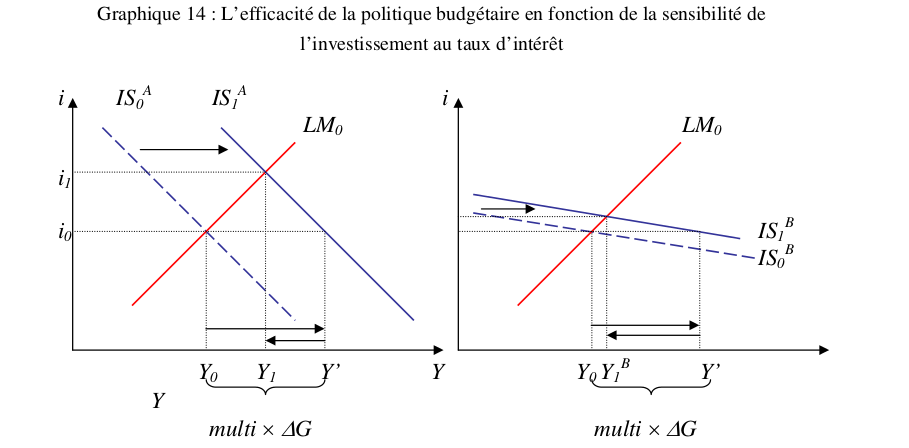
\includegraphics[width=12cm]{graph39.png}
\end{center}
Les deux économies ne se distinguent que par la pente de la courbe IS. On constate que l'effet d'éviction est plus important dans l'économie B que dans l'économie A, l'augmentation du revenu est donc plus faible dans l'économie B que dans l'économie A. \\
On peut donc en conclure que \textbf{la politique budgétaire est d'autant plus efficace que la valeur du multiplicateur est élevée et que l'investissement est peu sensible au taux d'intérêt}. \\
Si la forme de IS peut déterminer l'efficacité de la politique budgétaire c'est surtout sur le rôle du marché de la monnaie que les débats on porté puisque c'est l'augmentation du taux d'intérêt qui détermine l'ampleur de  l'effet d'éviction. Par conséquent, c'est la forme de LM qui joue le rôle principal. \\
Les deux paramètres qui déterminent la pente de la courbe LM sont la sensibilité au revenu de la demande de monnaie de transaction et la sensibilité au taux d'intérêt de la demande de monnaie de précaution et à des fins de spéculation. En effet, plus la demande de monnaie de transaction sera sensible au revenu, plus l'augmentation initiale du revenu provoquera une demande excédentaire de monnaie. L'augmentation du taux d'intérêt nécessaire pour résorber cette demande excédentaire sera donc plus importante, ce qui augmentera l'effet d'éviction. \\
Bien que la sensibilité de la demande de monnaie de transaction puisse influencer l'efficacité de la politique budgétaire, c'est sur le rôle de la sensibilité de la demande de monnaie au taux d'intérêt que les débats ont porté. En effet, une des principales différences entre les théories keynésiennes et classiques porte sur les déterminants de la demande de monnaie. \\
Pour les classiques, la monnaie d'est détenue que pour réaliser des transactions. Sa demande est donc insensible au taux d'intérêt. L4apport de la théorie keynésienne est d'avoir suggéré qu'il existait d'autres motifs de détention de la monnaie et que la demande de monnaie était donc insensible au taux d'intérêt. \\
On peut donc présenter l'opposition entre les théories keynésiennes et classiques comme le résultat d'un désaccord portant la pente de la courbe LM. Pour les classiques, cette courbe est verticale. Pour les keynésiens, elle est croissante, voire horizontale lorsque l'économie est en situation de trappe à liquidité. Comme le cas d'une courbe LM croissante a déjà été vu, on va se concentrer sur les deux cas extrêmes :
\begin{center}
  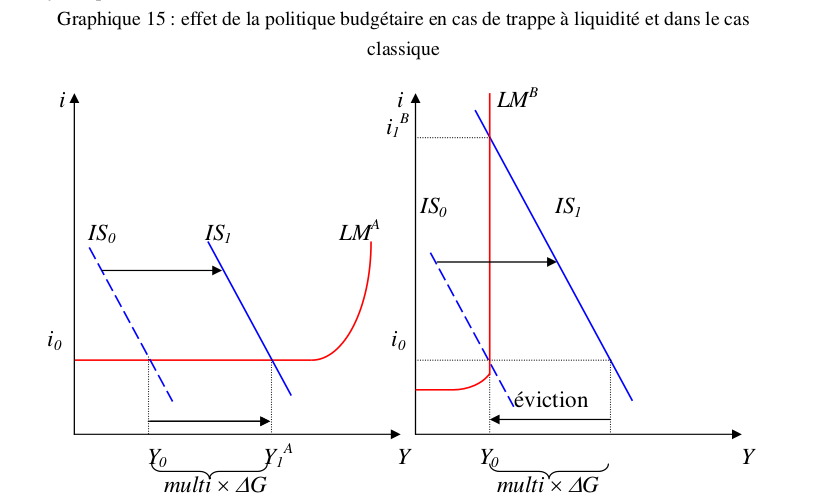
\includegraphics[width=12cm]{graph40.png}
\end{center}
Ce graphique présente l'effet d'une politique budgétaire de même ampleur dans deux économies qui partent de la même position mais se distinguent par la situation de leur marché de la monnaie : l'économie A est confrontée à une trappe à liquidité alors que l'économie B est en situation classique. \\
Dans l'économie A, on constate que la politique budgétaire provoque une augmentation du revenu correspondant à l'effet multiplicateur et que le taux d'intérêt reste constant. Dans cette économie, il n'y a donc par d'effet d'éviction et l'efficacité de la politique budgétaire est maximale. \\
En effet, comme l'économie est en situation de trappe à liquidité, le taux d'intérêt a atteint sa valeur minimum et la demande de monnaie est infiniment sensible au taux d'intérêt. L'augmentation de la demande de monnaie sera résorbée sans que le taux d'intérêt ait besoin de réagir. Comme le taux d'intérêt est constant, l'effet d'éviction sera nul. L'effet total de la politique budgétaire sera donc égal à l'effet multiplicateur. On peut donc conclure que \textbf{l'efficacité de la politique budgétaire est maximale lorsque l'économie est en situation de trappe à liquidité}. \\
La situation est toute différente dans l'économie B où la demande de monnaie est totalement insensible au taux d'intérêt. Dans cette économie, l'effet d'éviction compense totalement l'effet multiplicateur. \\
Dans cette économie, la politique budgétaire provoque une relance temporaire grâce à l'effet multiplicateur. Comme le revenu augmente, la demande de monnaie de transaction augmente, ce qui entraîne une demande excédentaire de monnaie. Le taux d'intérêt se met alors à augmenter, mais cette augmentation n'affecte pas la demande de monnaie. Elle affecte en revanche l'investissement qui se met à décroître. Comme l'investissement diminue, la demande globale diminue, ce qui réduit le revenu. La demande de monnaie de transaction diminue alors, ce qui réduit la demande excédentaire de monnaie, et ce mécanisme se poursuit tant qu'il y a une demande excédentaire de monnaie. \\
Le marché de la monnaie ne retourne à l'équilibre que lorsque la demande de monnaie de transaction a retrouvé son niveau initial, ce qui signifie que le revenu a aussi retrouvé son niveau initial. Par conséquent, la diminution de l'investissement a intégralement compensé l'augmentation initiale des dépenses publiques. On dit que les dépenses publiques ont évincé l'investissement privé. Le seul effet de la relance budgétaire est d'avoir fait augmenter le taux d'intérêt et réduit l'investissement. On peut donc conclure que \textbf{la politique budgétaire est totalement inefficace lorsque la demande de monnaie est insensible au taux d'intérêt}. \\
En comparant ces deux situation et en les complétant avec le cas standard, on peut donc affirmer que \textbf{la politique budgétaire est d'autant plus efficace que la demande de monnaie est sensible au taux d'intérêt}.
\subsection{Le policy-mix}
Les politiques budgétaires et monétaires peuvent être utilisées conjointement. Le policy-mix est le dosage des deux politiques.
\subsubsection{Politique budgétaire expansionniste accompagnée d'une politique monétaire restrictive}
On a vu qu'un politique budgétaire expansionniste se traduisait par un déplacement vers la droite de la courbe IS alors qu'une politique monétaire restrictive déplaçait la courbe LM vers le haut.
\begin{center}
  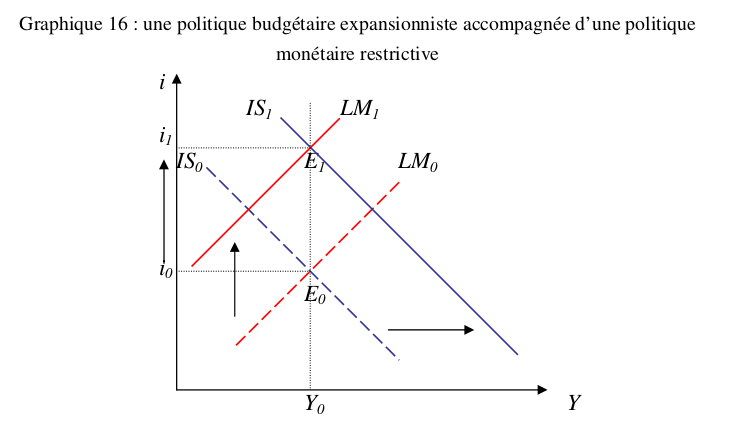
\includegraphics[width=12cm]{graph41.png}
\end{center}
La politique monétaire accentue l'effet d'éviction. Le taux d'intérêt augmente encore plus et le revenu encore moins qu'en présence d'une politique monétaire neutre. Dans le cas qui est représenté ci dessus, la politique monétaire contrecarre exactement la politique budgétaire, si bien que le revenu reste constant. \\
C'est un cas particulier. Si la politique monétaire était moins restrictive le revenu pourrait augmenter légèrement, et inversement si la politique monétaire était plus restrictive le revenu pourrait même diminuer. \\
Dans tous les cas un tel policy-mix est incohérent puisqu'il n'a aucun impact sur le revenu mais implique une augmentation inutile des dépenses et du taux d'intérêt. La situation initiale serait donc préférable puisque les dépenses seraient inférieures, ce qui permettrait de ne pas augmenter la dette publique sans que le revenu soit différent.
\subsubsection{Politique budgétaire expansionniste accompagnée d'une politique monétaire expansionniste}
Comme précédemment, la politique budgétaire est expansionniste et déplace donc la courbe IS vers la droite, mais la politique monétaire est à présent elle aussi expansionniste et déplace donc la courbe LM vers le bas.
\begin{center}
  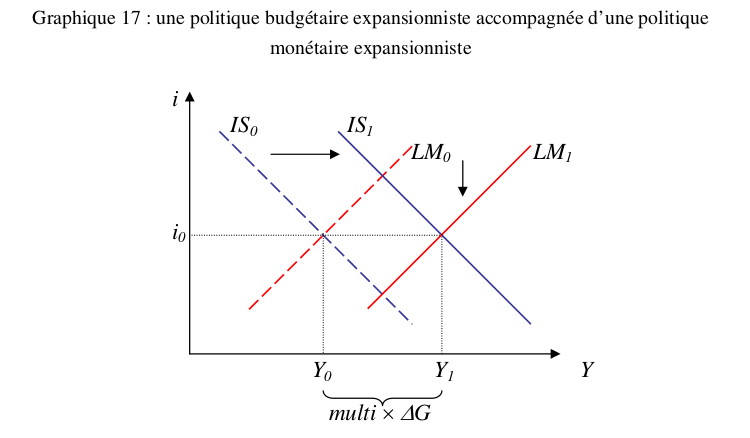
\includegraphics[width=12cm]{graph42.png}
\end{center}
On voit que dans ces conditions les deux effets se complètent et résultent en une augmentation du revenu accompagnée d'une hausse limitée du taux d'intérêt. Le graphique montre que la politique monétaire stabilise exactement le taux d'intérêt. L'effet d'éviction est ainsi évité et l'augmentation du revenu correspond exactement à l'effet multiplicateur. \\
Comme précédemment, il s'agit là d'un cas extrême. Plus généralement, on peut dire que lorsque la politique monétaire est expansionniste elle augmente l'efficacité de la politique budgétaire. L'augmentation du revenu est supérieure, et celle du taux d'intérêt inférieure, à celle qui aurait été constatée si la politique monétaire était restée passive. \\
Si on avait inversé les rôles et étudié une politique monétaire expansionniste confrontée à une politique budgétaire soit expansionniste, soit restrictive, on aurait obtenu des résultats comparables. \\
L'étude du policy-mix permet donc de conclure que \textbf{l'efficacité de la politique budgétaire dépend de la politique monétaire mise en oeuvre et vice versa}.


\appendix
\chapter{Notations} 
\begin{itemize}
  \item $PIB_{cf}$ : PIB au coût des facteurs
  \item $PIB_{pm}$ : PIB aux prix du marché
  \item $Y$ : PIB
  \item $C$ : Consommation
  \item $I$ : Investissement
  \item $S$ : Épargne
  \item $G$ : Dépenses publiques
  \item $NX$ : Exportations nettes des importations
  \item $T$ : Impôts
  \item $K$ : Capital
  \item $L$ : Travail
\end{itemize}


\end{document}

% LocalWords:  Keynes macroéconomiques micro-économiques NX S-I T-G déflateur
% LocalWords:  PNB IDH l'IPC i.e macroéconomiste Ricardo Solow néoclassique t-n
% LocalWords:  Phillips Friedman Dpub luxembourgeois PPA hédoniques l'ONEM PmC
% LocalWords:  David c.Y micro-économique market BC refinancement Refi TQM IS
% LocalWords:  néoclassiques tautologique d'hyperinflation l'hyperinflation LM
% LocalWords:  d'encaisses IS-LM Hicks Hansen policy-mix
